\documentclass[twoside,11pt]{article}

% Any additional packages needed should be included after jmlr2e.
% Note that jmlr2e.sty includes epsfig, amssymb, natbib and graphicx,
% and defines many common macros, such as 'proof' and 'example'.
%
% It also sets the bibliographystyle to plainnat; for more information on
% natbib citation styles, see the natbib documentation, a copy of which
% is archived at http://www.jmlr.org/format/natbib.pdf

\usepackage{jmlr2e}
% packages with special commands
\usepackage{amssymb, amsmath}
\usepackage{epsfig}
\usepackage{array}
\usepackage{ifthen}
\usepackage{color}
\usepackage{fancyhdr}
\usepackage{graphicx}
\usepackage{mathtools}
\usepackage{csquotes}
\usepackage{multirow}
\usepackage{xcolor}
\usepackage{chngcntr}
\usepackage{apptools}
\AtAppendix{\counterwithin{lemma}{section}}
%\usepackage[comma,authoryear]{natbib}

%\addbibresource{example.bib} % The filename of the bibliography



% Definitions of handy macros can go here
\newcommand{\skone}{\mathcal{S}_{k_1}}
\newcommand{\sktwo}{\mathcal{S}_{k_2}}

\newcommand{\tr}{\text{tr}}
\newcommand{\E}{\textbf{E}}
\newcommand{\diag}{\text{diag}}
\newcommand{\argmax}{\text{argmax}}
\newcommand{\Cov}{\text{Cov}}
\newcommand{\Var}{\text{Var}}
\newcommand{\argmin}{\text{argmin}}
\newcommand{\Vol}{\text{Vol}}
\newcommand{\comm}[1]{}
\newcommand{\indep}{\rotatebox[origin=c]{90}{$\models$}}
\newcommand{\Cor}{\text{Cor}}
\newcommand{\bZ}{\boldsymbol{Z}}
\newcommand{\bz}{\boldsymbol{z}}
\newcommand{\bx}{\boldsymbol{x}}
\newcommand{\bX}{\boldsymbol{X}}

\newcommand{\bH}{\boldsymbol{H}}


\newcommand{\fracpartial}[2]{\frac{\partial #1}{\partial  #2}}

\newenvironment{myfont}{\fontfamily{phv}\selectfont}{\par}

% Heading arguments are {volume}{year}{pages}{submitted}{published}{author-full-names}

\jmlrheading{0}{00}{0-00}{0/00}{00/00}{zheng00}{Charles Zheng and Rakesh Achanta and Yuval Benjamini}

% Short headings should be running head and authors last names

\ShortHeadings{Extrapolating expected accuracies}{Zheng, Achanta and Benjamini}
\firstpageno{1}

\begin{document}

\title{Extrapolating expected accuracies for recognition tasks}

\editor{No One Yet}

\author{\name Charles Zheng \email charles.y.zhang@gmail.com \\
       \addr Department of Statistics\\
       Stanford University\\
       Palo Alto, CA 
       \AND
       \name Rakesh Achanta \email  \\
       \addr Department of Statistics\\
       Stanford University\\
       Palo Alto, CA 
       \AND
       \name Yuval Benjamini \email yuval.benjamini@mail.huji.ac.il \\
       \addr Department of Statistics\\
       The Hebrew University of Jerusalem,\\
       Jerusalem, Israel}

\maketitle

\begin{abstract}%   <- trailing '%' for backward compatibility of .sty file
The difficulty of multi-class classification generally increases with
the number of classes.  Using data from a subset of the classes, can
we predict how well a classifier will scale with an increased number
of classes?  Under the assumption that the classes are sampled
identically and independently from a population, and under the
assumption that the classifier is based on independently learned
scoring functions, we show that the expected accuracy when the
classifier is trained on $k$ classes is the $k-1$st moment of a
certain distribution that can be estimated from data.  We present an
unbiased estimation method based on the theory, and demonstrate its
application on a facial recognition example.
\end{abstract}

\begin{keywords}
Multiclass classification
\end{keywords}
\section{Introduction}\label{sec:recog_tasks}

Many machine learning tasks are interested in recognizing or
identifying an individual instance within a large set of possible
candidates. These problems are usually modeled as multi-class
classification problems, with a large and possibly complex label
set. Leading examples include detecting the speaker from his voice
patterns \citep{togneri2011overview}, identifying the author from her
written text \citep{stamatatos2014overview}, or labeling the object
category from its image
\citep{duygulu2002object,deng2010does,oquab2014learning}.  In all
these examples, the algorithm observes an input $x$, and uses the
classifier function $h$ to guess the label $y$ from a large label set
$\mathcal{S}$.

There are multiple practical challenges in developing recognition
systems for large label sets. Collecting high quality training data is
perhaps the main obstacle, as the costs scale with the number of
classes.  It can be affordable to first collect data for a small set
of classes, even if the long-term goal is to generalize to a larger
set.  Furthermore, classifier development can be accelerated by
training first on fewer classes, as each training cycle may require
substantially less resources.  Indeed, due to interest in how
small-set performance generalizes to larger sets, such comparisons can
found in the literature \citep{oquab2014learning, griffin2007caltech}.
A natural question is how does changing the size of the label set
affect the classification accuracy?

Technically, we consider a pair of classification problems on finite
label sets: a source task with label set $\mathcal{S}_{k_1}$ of size
$k_1$, and a target task with a larger label set $\mathcal{S}_{k_2}$
of size $k_2 > k_1$.  For each label set $\mathcal{S}_k$, one
constructs the classification rule $h^{(k)}:\mathcal{X} \to
\mathcal{S}_{k}$.  Supposing that in each task, the test example
$(X^*, Y^*)$ has a joint distribution, define the generalization
accuracy for label set $\mathcal{S}_k$ as
\begin{equation}\label{eq:ga_k}
\text{GA}_k = \Pr[h^{(k)}(X^*) = Y^*].
\end{equation}
The problem of \emph{performance extrapolation} is the following:
using data from only the source task $\mathcal{S}_{k_1}$, 
predict the accuracy for a target task with a larger unobserved 
label set $\mathcal{S}_{k_2}$.

A natural use case for performance extrapolation would be in the
deployment of a facial recognition system.  Suppose a system was
developed in the lab on a database of $k_1$ individuals. Clients would
like to deploy this system on a new larger set of $k_2$
individuals. Performance extrapolation could allow the lab to predict
how well the algorithm will perform on the client's problem,
accounting for the difference in label set size.

Extrapolation should be possible when the source and target
classifications are two instances of the same recognition problem.  In
many cases, the set of categories $\mathcal{S}$ is to some degree a
random or arbitrary selection out of a larger, perhaps infinite, set
of potential categories $\mathcal{Y}$. Yet any specific experiment
uses a fixed finite set.  For example, categories in the classical
Caltech-256 image recognition dataset \citep{griffin2007caltech} were
assembled by aggregating keywords proposed by students and then
collecting matching images from the web.  The arbitrary nature of the
label set is even more apparent in biometric applications (face
recognition, authorship, fingerprint identification) where the labels
correspond to human individuals \citep{togneri2011overview,
  stamatatos2014overview}.  In all these cases, the number of the
labels used to define a concrete dataset is therefore an experimental
choice rather than a property of the domain.  Despite the arbitrary
nature of these choices, such datasets are viewed as representing the
larger problem of recognition within the given domain, in the sense
that success on such a dataset should inform performance on similar
problems.

In this paper, we model the label sets as randomly sampled from some
population.  Not only does the assumption of randomness capture the
ambiguity of actual label sets, but it also provides a powerful
formalism for answering the question of how to extrapolate.
Furthermore, we assume that both $\mathcal{S}_{k_1}$ and
$\mathcal{S}_{k_2}$ are independent identically distributed (i.i.d.)
samples from a population (or distribution) of labels $ \pi$, which is
defined on the label space $\mathcal{Y}$.  Since the label set is
random, the generalization accuracy of a given classifier becomes a
random variable.  Performance extrapolation then becomes the problem
of estimating the average generalization accuracy $\text{AGA}_k$ of an
i.i.d. label set $\mathcal{S}_k$ of size $k$.  The condition of
i.i.d. sampling of labels ensures that the separation of labels in a
random set $\mathcal{S}_{k_2}$ can be inferred by looking at the
empirical separation in $\mathcal{S}_{k_1}$, and therefore that some
estimate of the average accuracy on $\mathcal{S}_{k_2}$ can be
obtained.  We also make the assumption that the classifiers train a
separate model for each class.  This convenient property allows us to
characterize the accuracy of the classifier by selectively
conditioning on one class at a time.

Our paper presents two main contributions.  The first is a formula for
calculating the $k$-class average accuracy of a marginal classifier.
The only unknown quantity in the formula is a function ${D}$ which
is determined by properties of the data distribution and the
classifier.  The second is a method for extrapolating the average
accuracy curve from $k_1$-class data to a larger number of classes.
The method is based on estimating the unknown function ${D}$, and
under certain conditions it has the property of being an unbiased
estimator of the average accuracy.

The paper is organized as follows.  In the rest of this section, we
discuss related work.  The framework of randomized classification is
introduced in Section \ref{sec:rc_motivation}, and there we also
introduce a toy example which is revisited throughout the
paper. Section \ref{sec:extrapolation} develops our theory of
extrapolation, and Section \ref{sec:extrapolation_estimation} we
suggest an estimation method. In Section
\ref{sec:extrapolation_example}, we demonstrate our method on a facial
recognition problem, making use of the OpenFace feature extraction
network \cite{amos2016openface}. In Section \ref{sec:discussion} we
discuss modeling choices and limitations of our theory, as well as
potential extensions.

\subsection{Related work}

Most existing works on classification for large label sets deal with the
computational challenges of jointly optimizing the many parameters
required for these models: \citep{crammer2001algorithmic,
  lee2004multicategory, weston1999support} are tied to a
specific algorithm for classification, whereas \cite{gupta2014training}
present a method for estimating the accuracy of a classifier which can
be used to improve performance for general classifiers.

Linking performance between two different but related classification
tasks can be considered an instance of transfer learning
\citep{pan2010survey}. Under \citeauthor{pan2010survey}'s terminology,
our setup is an example of multi-task learning, because the source
task has labeled data, which is used to predict performance on a
target task that also has labeled data.  Examples of transfer learning
from one label set to another include \cite{oquab2014learning},
\cite{donahue2014decaf}, \cite{sharif2014cnn}.

An example that deals with extrapolation of classification error to a
larger number of classes can be found in \cite{Kay2008a}. They tested
a model for classifying natural images based on a subject's fMRI brain
scan, achieving over 0.75 accuracy of classification on a set of $k_1
= 1000$ natural stimuli. From these results, they estimated the
maximum size of the stimuli set before the model accuracy drops below
0.10. Specifically, they estimated the density function of
incorrect-label scores for each example in the test dataset, and then
computed the probability of correct classification assuming that
future labels were drawn from the estimated density.  However, as we
will discuss, their method suffers from bios due to failing to account
for the error in the estimated density.

The theoretical framework we adopt is one where there exists a family
of classification problems with increasing number of classes. This
framework can be traced back to \cite{Shannon1948}, who considered the
error rate of a random codebook, which is a special case of randomized
classification. More recently, a number of authors have considered the
problem of high-dimensional feature selection for multiclass
classification with a large number of classes \citep{pan2016ultrahigh,
  abramovich2015feature, davis2011bayesian}.  All of these works
assume specific distributional models for classification compared to
our more general setup. However, we do not deal with the problem of
feature selection.

\section{Randomized classification}\label{sec:rc_motivation}


\subsection{Setup}

The randomized classification model we study has the following
features.  We assume that there exists an infinite, perhaps
continuous, label space $\mathcal{Y}$ and a example space $\mathcal{X}
\in \mathbb{R}^p$.  We assume there exists a prior distribution $\pi$
on the label space $\mathcal{Y}$.  And for each label $y \in
\mathcal{Y}$, there exists a distribution of examples $F_y$. In other
words, for an example-label pair $(X, Y)$, the conditional
distribution of $X$ given $Y = y$ is given by $F_y$.
%Furthermore, we assume that
%there exists a prior distribution $\pi$ on the label space $\mathcal{Y}$.

A random classification task can be generated as follows.  The label
set $\mathcal{S} = \{Y^{(1)},\hdots, Y^{(k)}\}$ is generated by
drawing labels $Y^{(1)},\hdots, Y^{(k)}$ i.i.d. from $\pi$.  For each
label, we sample a training set and a test set.  The training set is
obtained by sampling $r_{train}$ observations $X_{j, train}^{(i)}$
i.i.d. from $F_{Y^{(i)}}$ for $j = 1,\hdots, r_{train}$ and $i =
1,\hdots, k$.  The test set is likewise obtained by sampling $r$
observations $X_j^{(i)}$ i.i.d. from $F_{Y^{(i)}}$ for $j = 1,\hdots,
r$.

We assume that the classifier $h(x)$ works by assigning a score to
each label $y^{(i)} \in \mathcal{S}$, then choosing the label with the
highest score.  That is, there exist real-valued \emph{score
  functions} $m_{y^{(i)}}(x)$ for each label $y^{(i)} \in
\mathcal{S}$.  Since the classifier is allowed to depend on the
training data, it is convenient to view it (and its associated score
functions) as random.  We write $H(x)$ when we wish to work with the
classifier as a random function, and likewise $M_y(x)$ to denote the
score functions when they are considered as random.

For a fixed instance of the classification task with labels
$\mathcal{S} = \{y^{(i)}\}_{i=1}^k$ and associated score functions
$\{m_{y^{(i)}}\}_{i=1}^k$, recall the definition of the $k$-class
generalization error \eqref{eq:ga_k}.  Assuming that there are no
ties, it can be written in terms of score functions as
\[
\text{GA}_k(h) = \frac{1}{k} \sum_{i=1}^k  \Pr[m_{y^{(i)}}(X^{(i)}) = \max_j
m_{y^{(j)}}(X^{(i)})],
\]
where $X^{(i)} \sim F_{y^{(i)}}$ for $i =1,\hdots, k$.  However, when
we consider the labels $\{Y^{(i)}\}_{i=1}^k$ and associated score
functions to be random, the generalization accuracy also becomes a
random variable.

Suppose we specify $k$ but do not fix any of the random quantities in
the classification task.  Then the $k$-class \emph{average
  generalization accuracy} of a classifier is the expected value of
the generalization accuracy $\text{GA}_k(H)$ resulting from a random
set of $k$ labels, $Y^{(1)}, \hdots, Y^{(k)} \stackrel{iid}{\sim
  \pi}$, and their associated score functions:
\begin{align*}
\text{AGA}_k &= \frac{1}{k} \sum_{i=1}^k \Pr[M_{Y^{(i)}}(X^{(i)}) = \max_j
M_{Y^{(j)}}(X^{(i)})]
\\&= \Pr[M_{Y^{(1)}}(X^{(1)}) = \max_j M_{Y^{(j)}}(X^{(1)})].
\end{align*}
The last line follows from noting that all $k$ summands in the
previous line are identical.  [The definition of average
  generalization accuracy is illustrated in Figure
  \ref{fig:average_risk}.]

\begin{figure}[h]
\centering
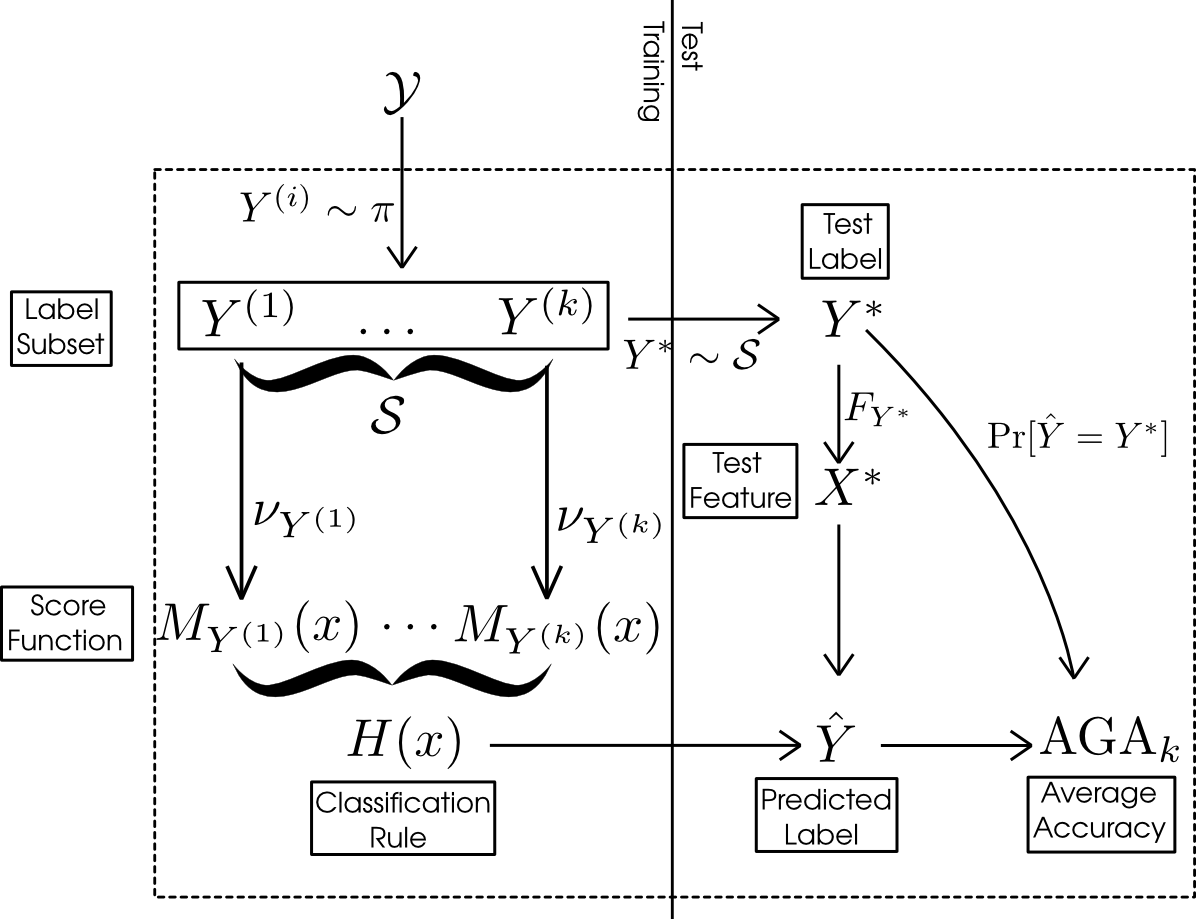
\includegraphics[scale = 0.3]{average_risk.png}
\caption{\textbf{Average generalization accuracy:} A diagram of the random quantities underlying the average generalization accuracy for $k$ labels ($\text{AGA}_k$). At the training stage (left), a set of $k$ labels $\mathcal{S}$ is sampled from the prior $\pi$, and score functions are trained from examples for these classes. At the test stage (right), one true class $Y^*$ is sampled uniformly from $\mathcal{S}$, as well as a test example $X^*$. $\text{AGA}_k$ measures the expected accuracy over these random variables.}\label{fig:average_risk}
\end{figure}

\subsubsection{Marginal classifier}

In our analysis, we do not want the classifier to rely too strongly on
complicated interactions between the labels in the set. We therefore
propose the following property of marginal separability for
classification models:

\begin{definition}
The classifier $H(x)$ is called a \emph{marginal classifier} if the
score function $M_{y^{(i)}}(x)$ only depends on the label $y^{(i)}$
and the class training set $X_{j, train}^{(i)}$.
\[M_{y^{(i)}}(x) = g(x; y^{(i)},X_{1, train}^{(i)},...,X_{r_{train}, train}^{(i)})\]
\end{definition}
This means that the score function for $y^{(i)}$ does not depend on
other labels $y^{(j)}$ or their training samples.  Therefore, each
$M_y$ can be considered to have been drawn from a distribution
$\nu_y$.  Classes ``compete'' only through selecting the highest
score, but not in constructing the score functions.  The operation of
a marginal classifier is illustrated in figure
\ref{fig:classification_rule}.


\begin{figure}[h]
\centering
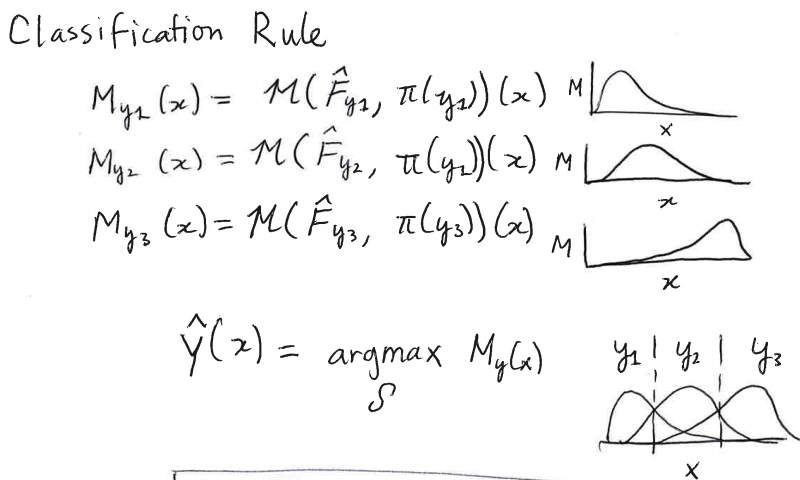
\includegraphics[scale = 0.4]{classification_rule.png}
\caption{\textbf{Classification rule:} Top: Score functions for three classes for a one-dimensional example space. Bottom: The classification rule chooses between $y^{(1)},y^{(2)}$ or $y^{(3)}$ by choosing the maximal score function. 
%A classifier is marginal if each score function does not depend on labels or training samples for other classes. 
}
\label{fig:classification_rule}
\end{figure}

The \emph{marginal} property allows us to prove
strong results about the accuracy of the classifier under
i.i.d. sampling assumptions.


\textbf{Comments:}
\begin{enumerate}
\item If $H$ is a marginal classifier then 
$M_{Y^{(i)}}$ is independent of $Y^{(j)}$ and $M_{Y^{(j)}}$ for $i \neq j$.
\item Estimated Bayes classifier are a primary example of a marginal
  classifier. Let $\hat{f_y}$ be a density estimate of the example
  distribution under label $y$ obtained from the empirical
  distribution $\hat{F_y}$. Then, we can use the estimated density to
  produce the score functions:
\[ m^{EB}_y(x) = \log(\hat{f_{y}}(x)).\]
The resulting empirical approximation for the Bayes classifier would
be
\[ h^{EB}(x) = \text{argmax}_{y \in \mathcal{S}}(m^{EB}_y(x)).\]
\item Both the Quadratic Discriminant Analysis and the naive Bayes
  classifiers can be seen as specific instances of an estimated Bayes
  classifier
\footnote{QDA is the special case of the estimated Bayes classifier
  when $\hat{f_y}$ is obtained as the multivariate Gaussian density
  with mean and covariance parameters estimated from the data.  Naive
  Bayes is the estimated Bayes classifier when $\hat{f_y}$ is obtained
  as the product of estimated componentwise marginal distributions of
  $p(x_i|y)$}.  For QDA, the score function is given by
\[
m_y^{QDA}(x) = -(x - \mu(\hat{F}_y))^T \Sigma(\hat{F}_y)^{-1} (x-\mu(\hat{F}_y)) - \log\det(\Sigma(\hat{F}_y)),
\]
where $\mu(F) = \int y dF(y)$ and $\Sigma(F) = \int (y-\mu(F))(y-\mu(F))^T dF(y)$.
In Naive Bayes, the score function is
\[
m^{NB}_y(x) = \sum_{j=1}^p \log \hat{f}_{y, j}(x),
\]
where $\hat{f}_{y, j}$ is a density estimate for the $j$-th component of
$\hat{F}_y$.
\item For some classifiers, $M_y$ is a deterministic function of $y$
  (and therefore $\nu_y$ is degenerate). A prime example is when
  exists fixed or pre-trained embeddings $g, \tilde{g}$ that map
  labels $y$ and examples $x$ into $R^p$. Then
\begin{equation}
M_y^{embed} = -\|g(y) - \tilde{g}(x)\|_2.
\end{equation}
This describes, for example, a 1-nearest neighbor classifier.
\item There are many classifiers which do not satisfy the marginal
  property, such as multinomial logistic regression, multilayer neural
  networks, decision trees, and k-nearest neighbors.
\end{enumerate}

\emph{Notational remark.}  Henceforth, we shall relax the assumption
that the classifier $H(x)$ is based on a training set.  Instead, we
assume that there exist score functions $\{M_{Y^{(i)}}\}_{i=1}^k$
associated with the random label set $\{Y^{(i)}\}_{i=1}^k$, and that
the score functions $M_{Y^{(i)}}$ are independent of the test set.
The classifier $H(x)$ is marginal if and only if $M_{Y^{(i)}}$ are
independent of both $Y^{(j)}$ and $M_{Y^{(j)}}$ for $j \neq i$.

\subsection{Estimation of average accuracy}\label{sec:estimation_average_accuracy}

Suppose we have test data for a classification task with $k_1$
classes.  That is, we have a label set $\mathcal{S}_{k_1} =
\{y^{(i)}\}_{i=1}^{k_1}$ and its associated set of score functions
$M_{y^{(i)}}$, as well as test observations $(x_1^{(i)},\hdots,
x_{r}^{(i)})$ for $i = 1,\hdots, k_1$.  What would be the predicted
accuracy for a new randomly sampled set of $k_2 \leq k_1$ labels?

Note that $\text{AGA}_{k_2}$ is the expected value of the accuracy on
the new set of $k_2$ labels.  Therefore, any unbiased estimator of
$\text{AGA}_{k_2}$ will be an unbiased predictor for the accuracy on
the new set.

Let us start with the case $k_2 = k_1 = k$.  For each test observation
$x_j^{(i)}$, define the ranks of the candidate classes $\ell =
1,\hdots, k$ by
\[
R_{j}^{i, \ell} = \sum_{s = 1}^k I\{m_{y^{(\ell)}}(x_j^{(i)}) \geq m_{y^{(s)}}(x_j^{(i)})\}.
\]
The test accuracy is the fraction of observations for which the
correct class also has the highest rank
\begin{equation}\label{eq:test_risk}
\text{TA}_k = \frac{1}{r k} \sum_{i=1}^{k} \sum_{j=1}^{r} I\{R_j^{i,i} = k\}.
\end{equation}
Taking expectations over both the test set and the random labels, the
expected value of the test accuracy is $\text{AGA}_k$; hence,
$\text{TA}_k$ provides the desired estimator.

Next, let us consider the case where $k_2 < k_1$.  Consider label set
$\mathcal{S}_{k_2}$ obtained by sampling $k_2$ labels uniformly
without replacement from $\mathcal{S}_{k_1}$. Since
$\mathcal{S}_{k_2}$ is unconditionally an i.i.d. sample from the
population of labels $\pi$, the test accuracy of $\mathcal{S}_{k_2}$
is an unbiased estimator of $\text{AGA}_{k_2}$.  However, we can get a
better unbiased estimate of $\text{AGA}_{k_2}$ by averaging over all
the possible subsamples $\mathcal{S}_{k_2} \subset \mathcal{S}_{k_1}$.
This defines the average test accuracy over subsampled tasks,
$\text{ATA}_{k_2}$.

\emph{Remark.}  Na\"{i}vely, computing $\text{ATA}_{k_2}$ requires us
to train and evaluate ${k_1}\choose{k_2}$ classification rules.
However, for marginal classifiers, retraining the classifier is not
necessary.  Looking at the rank $R_{j}^{i,i}$ of the correct label $i$
for $x_j^{(i)}$, allows us to determine how many subsets
$\mathcal{S}_2$ will result in a correct classification. Specifically,
there are $R_{j}^{i,i} - 1$ labels with a lower score than the correct
label $i$.  Therefore, as long as one of the classes in
$\mathcal{S}_2$ is $i$, and the other $k_2-1$ labels are from the set
of $R_{j}^{i,i}-1$ labels with lower score than $i$, the
classification of $x_j^{(i)}$ will be correct.  This implies that
there are ${R_{j}^{i,i}-1}\choose{k_2-1}$ such subsets $\mathcal{S}_2$
where $x_j^{(i)}$ is classified correctly, and therefore the average
test risk for all ${k_1}\choose{k_2}$ subsets $\mathcal{S}_2$ is
\begin{equation}\label{eq:avtestrisk}
\text{ATA}_{k_2} = \frac{1}{{{k_1}\choose{k_2}}}\frac{1}{r k_2} \sum_{i=1}^{k_1} \sum_{j=1}^{r} {{R_{j}^{i,i}-1}\choose{k_2-1}}.
\end{equation}

\subsection{Toy Example: Bivariate normals}
\label{sec:toyExA}

Let us illustrate these ideas using a toy example.  Let $(Y, X)$ have
a bivariate normal joint distribution,
\[
(Y, X) \sim N\left(\begin{pmatrix}0 \\0\end{pmatrix}, \begin{pmatrix}1 & \rho \\ \rho & 1\end{pmatrix}\right),
\]
as illustrated in figure \ref{fig:toy1}(a).  Therefore, for a given
randomly drawn label $Y$, the conditional
distribution of $X$ for that label is univariate normal with mean $\rho Y$ and variance $1-\rho^2$:
\[
X|Y = y \sim N(\rho Y, 1-\rho^2).
\]
Supposing we draw $k = 3$ labels $y_1,y_2, y_3$, the classification
problem will be to assign a test instance $X^*$ to the correct label.
The test instance $X^*$ would be drawn with equal probability from one
of three conditional distributions $ X | Y=y^{(i)}$, as illustrated in
figure \ref{fig:toy1}(b, top).  The Bayes rule assigns $X^*$ to the
class with the highest density $p(x|y_i)$, as illustrated by figure
\ref{fig:toy1}(b, bottom): it is therefore a marginal classifier, with
score function
\[
M_{y^{(i)}}(x) = \log(p(x|y^{(i)})) = -\frac{(x - \rho y)^2}{2(1-\rho^2)}  + \text{const.}
\]

\begin{figure}[h]
\centering
\begin{tabular}{cc}
\begin{myfont}Joint distribution of $(X, Y)$\end{myfont} & 
\begin{myfont}Problem instance with $k = 3$\end{myfont}\\
\multirow{3}{*}{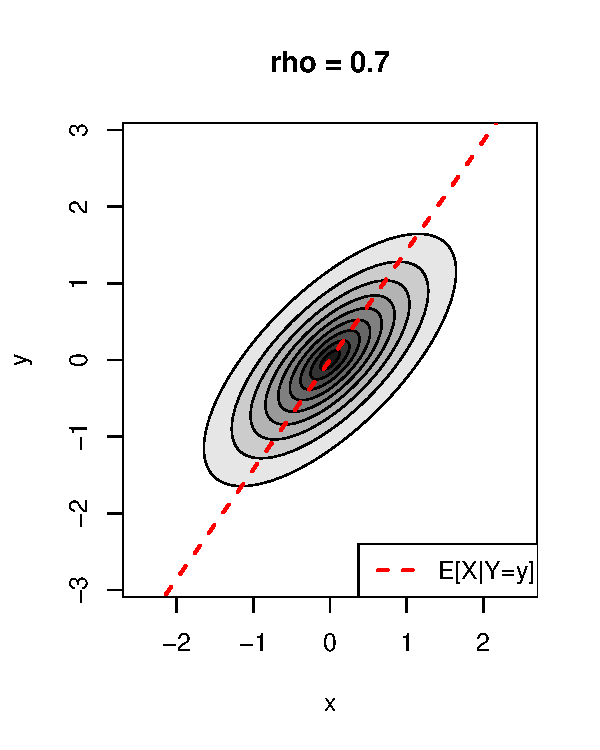
\includegraphics[scale = 0.5, clip = true, trim = 0 0 0 0.5in]{illus_rho_0_7.pdf}} & \\
& 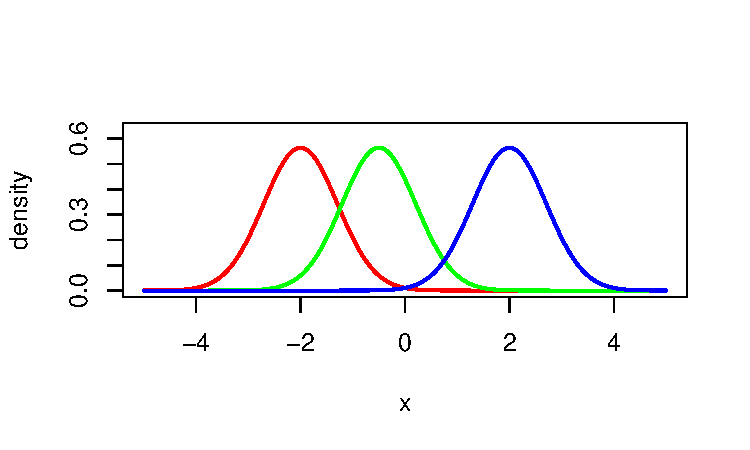
\includegraphics[scale = 0.5, clip = true, trim = 0 0.8in 0 0.8in]{illus_example1a.pdf}\\
 &  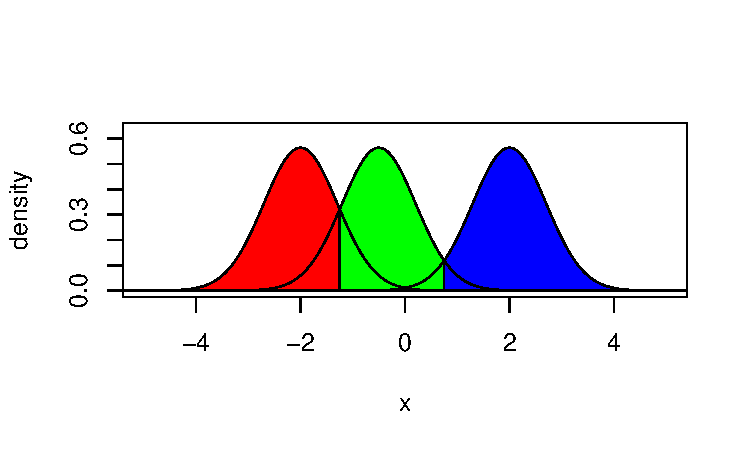
\includegraphics[scale = 0.5, clip = true, trim = 0 0 0 0.5in]{illus_example1b.pdf}\\
(a) & (b)
\end{tabular}

\caption{\textbf{Toy example:}
\emph{Left:} The joint distribution of $(X, Y)$ is bivariate normal with correlation $\rho = 0.7$.
\emph{Right:} A typical classification problem instance from the bivariate normal model with $k = 3$ classes.
\emph{(Top):} the conditional density of $X$ given label $Y$, for $Y = \{y^{(1)}, y^{(2)}, y^{(3)}\}$.
\emph{(Bottom):} the Bayes classification regions for the three classes.}\label{fig:toy1}
\end{figure}

For this model, the generalization accuracy of the Bayes rule for any
label set $\{y^{(1)},\hdots, y^{(k)}\}$ is given by
\begin{align*}
\text{GA}_k(y_1,\hdots, y_k) &= \frac{1}{k}\sum_{i=1}^k \Pr_{X \sim p(x|y_i)}[p(X|y_i) = \max_{j=1}^k p(X|y_j)]
\\&= \frac{1}{k}\sum_{i=1}^k \Phi\left(\frac{y^{[i+1]} - y^{[i]}}{2\sqrt{1-\rho^2}}\right) - \Phi\left(\frac{y^{[i-1]} - y^{[i]}}{2\sqrt{1-\rho^2}}\right)
\end{align*}
where $\Phi$ is the standard normal cdf, $y^{[1]} < \cdots < y^{[k]}$
are the sorted labels, and $y^{[0]} = -\infty$ and $y^{[k+1]} =
\infty$.  We numerically computed $\text{GA}_k(y_1,\hdots, y_k)$ for
randomly drawn labels $Y_1,\hdots, Y_k \stackrel{iid}{\sim} N(0, 1)$;
the distributions of $\text{GA}_k$ for $k = 2,\hdots, 10$ are
illustrated in figure \ref{fig:toy2}.  The mean of the distribution of
$\text{GA}_k$ is the $k$-class average risk, $\text{AGA}_k$. The
theory presented in the next section deals with how to analyze the
average risk $\text{AGA}_k$ as a function of $k$.


\begin{figure}[h]
\centering
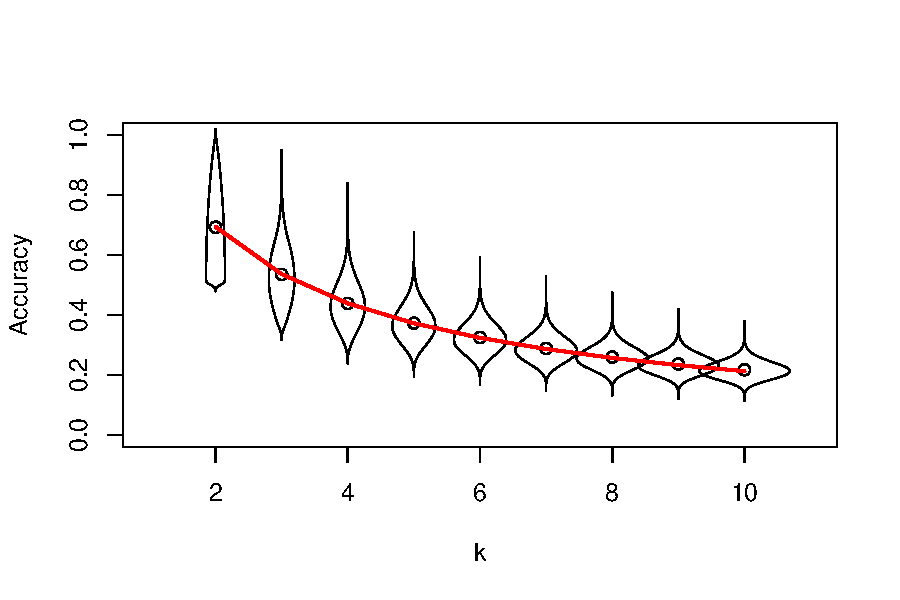
\includegraphics[scale = 0.7, clip = true, trim = 0 0 0 0.5in]{illus_err_0_7.pdf}

\caption{\textbf{Generalization accuracy for toy example:} The distribution of the generalization accuracy
  for $k = 2,3,\hdots, 10$ for the bivariate normal model with $\rho =
  0.7$.  Circles indicate the average generalization accuracy $\text{AGA}_k$; the red
  curve is the theoretically computed average accuracy.}\label{fig:toy2}
\end{figure}
\section{Extrapolation}
\label{sec:extrapolation}

The section is organized as follows.  We begin by introducing an
explicit formula for the average accuracy $\text{AGA}_{k}$.  The
formula reveals that $\text{AGA}_{k}$ is determined by moments of a
one-dimensional function ${D}(u)$.  Through this formula,
therefore, we can infer through subsample accuracies estimates of
${D}(u)$.  These estimates allow us to extrapolate the average
generalization accuracy to an arbitrary number of labels.

The result of our analysis is to expose the average accuracy
$\text{AGA}_{k}$ as the weighted average of a function ${D}(u)$,
where ${D}(u)$ is independent of $k$, and where $k$ only changes
the weighting.  The result is stated as follows.

\begin{theorem}\label{theorem:avrisk_identity}
Suppose $\pi$, $\{F_y\}_{y \in \mathcal{Y}}$ and score functions $M_y$
satisfy the tie-breaking condition.  Then, there exists a cumulative
distribution function ${D}(u)$ defined on the interval $[0,1]$
such that
\begin{equation}\label{eq:avrisk_identity}
\text{AGA}_{k} = 1 - (k-1) \int {D}(u) u^{k-2} du.
\end{equation}
\end{theorem}

The tie-breaking allows us
to neglect specifying the case when
margins are tied.
\begin{definition}
\emph{Tie-breaking condition}: for all $x \in \mathcal{X}$,
$M_Y(x) \neq M_{Y'}(x)$
with probability one for $Y, Y'$ independently drawn from $\pi$.
\end{definition}
In practice, one can simply break ties randomly,
which is mathematically equivalent to adding a small amount of random
noise $\epsilon$ to the function $\mathcal{M}$.

\subsection{Analysis of average accuracy}

For the following discussion, we often consider a random label with
its associated score function and example vector. Explicitly, this
sampling can be written:
\[Y \sim \pi,\, M_{Y}|Y \sim \nu_{Y},\, X|Y \sim F_{Y}. \]
%\[Y^* \sim \pi,\, M_{Y^*}|Y^* \sim \nu_{Y^*},\, X^*|Y^* \sim F_{Y^*},\, \]
%\[Y' \sim \pi,\, M_{Y'}|Y' \sim \nu_{Y'}\, X'|Y' \sim F_{Y'},\, \]
Similarly we use $(Y',M_{Y'},X')$ and $(Y^*,M_{Y^*},X^*)$ for two more
triplets with independent and identical distributions. Specifically,
$X^*$ will typically note the test example, and therefore $Y^*$ the
true label and $M_{Y^*}$ its score function.

The function ${D}$ is related to a favorability
function. Favorability measures the probability that the score for the
example $x^*$ is going to be maximized by the score function $m_y$,
compared to a random competitor $M_{Y'}$.  Formally, we write:
\begin{equation}\label{eq:U_function}
U_{x^*}(m_{y}) = \Pr[m_{y}(x^*) > M_{Y'}(x^*)].
\end{equation}

Note that for fixed example $x^*$, favorability is monotonically
increasing in $m_{y}(x^*)$.  If $m_y(x^*) > m_{y^\dagger}(x^*)$, then
$U_{x^*}(y) > U_{x^*}(y^\dagger)$, because the event $\{m_{y}(x^*) >
M_{Y'}(x^*)\}$ contains the event $\{m_{y^\dagger}(x^*) >
M_{Y'}(x^*)\}$.

Therefore, given labels $y^{(1)},\hdots,y^{(k)}$ and test instance
$x^*$, we can think of the classifier as choosing the label with the
greatest favorability:
\[
\hat{y} = \argmax_{y^{(i)} \in \mathcal{S}} m_{y^{(i)}}(x^*) = \argmax_{y^{(i)} \in \mathcal{S}} U_{x^*}(m_{y^{(i)}}).
\]
Furthermore, via a conditioning argument, we see that this is still
the case even when the test instance and labels are random:
\[
\hat{Y} = \argmax_{Y^{(i)} \in \mathcal{S}} M_{Y^{(i)}}(X^*) = \argmax_{Y^{(i)} \in \mathcal{S}} U_{X^*}(M_{Y^{(i)}}).
\]


The favorability takes values between 0 and 1, and when any of its
arguments are random, it becomes a random variable with a distribution
supported on $[0,1]$.  In particular, we consider the following two
random variables:
\begin{itemize}
\item[a.] the \emph{incorrect-label} favorability $U_{x^*}(M_Y)$
  between a given fixed test instance $x^*$, and the score function of
  a random incorrect label $M_{Y}$, and
\item[b.] the \emph{correct-label} favorability $U_{X^*}(M_{Y^*})$
  between a random test instance $X^*$, and the score function of the
  correct label, $M_{Y^*}$.
\end{itemize}
\subsubsection{Incorrect-label favorability}
The incorrect-label favorability can be written explicitly as
\begin{equation}
U_{x^*}(M_Y) = \Pr[M_{Y}(x^*) > M_{Y'}(x^*)|M_{Y}].
\end{equation}
Note that $M_Y$ and $M_{Y'}$ are identically distributed, and are both
are unrelated to $x^*$ that is fixed. This leads to the following
result:
\begin{lemma}\label{lemma:U_function}
Under the tie-breaking condition, the incorrect-label favorability
$U_{x^*}(M_Y)$ is uniformly distributed for any $x^* \in \mathcal{X}$,
and \begin{equation}\label{eq:Uniform} \Pr[U_{x^*}(M_Y) \leq u] = u.
\end{equation}
\end{lemma}
Proof is in the appendix. 

\subsubsection{Correct-label favorability}

The correct-label favorability is 
\begin{equation}
U^* = U_{X^*}(M_{Y^*}) = \Pr[M_{Y^*}(X^*) > M'_{Y'}(X^*)|Y^*,M_{Y^*},X^*].
\end{equation}
The distribution of $U^*$ will depend on $\pi$, $F_y$ and $\nu_y$, and
generally cannot be written in a closed form.  However, this
distribution is central to our analysis--indeed, we will see that the
function ${D}$ appearing in theorem \ref{theorem:avrisk_identity}
is defined as the cumulative distribution function of $U^*$.

The special case of $k=2$ shows the relation between the distribution
of $U^*$ and the average generalization accuracy, $\text{AGA}_2$. In
the two-class case, the average generalization accuracy is the
probability that a random correct label score function gives a larger
value than a random distractor:
\[
\text{AGA}_2 = \Pr[M_{Y^*}(X^*) > M_{Y'}(X^*)].
\]
where $Y^*$ is the correct label, and $Y'$ is a random incorrect
label.  If we condition on $Y^* = y^*$, $M_{Y^*} = m_{y^*}$ and $X^* =
x^*$, we get
\[
\text{AGA}_2 = \E[\Pr[M_{Y^*}(X^*) > M_{Y'}(X^*)|Y^*, M_{Y^*}, X^*]].
\]
Here, the conditional probability inside the expectation is the
correct-label favorability.  Therefore,
\[
\text{AGA}_2 = \E[U^*] = \int {D}(u) du,
\]
where ${D}(u)$ is the cumulative distribution function of $U^*$,
${D}(u) = \Pr[U^* \leq u]$.  Theorem \ref{theorem:avrisk_identity}
extends this to general $k$; we now give the proof.\newline


\noindent\textbf{Proof of Theorem \ref{theorem:avrisk_identity}}.

Without loss of generality, suppose that the true label is $Y^*$ and
the incorrect labels are $Y^{(1)},\hdots, Y^{(k-1)}$.  We have
\[
\text{AGA}_k = \Pr[M_{Y^*}(X^*) > \max_{i=1}^{k-1} M_{Y^{(i)}}(X^*)]
= \Pr[U^* > \max_{i=1}^{k-1} U_{X^*}(M_{Y^{(i)}})]
\]
recalling that $U^* = U_{X^*}(M_{Y^*})$.  Now, if we condition on $X^*
= x^*$, $Y^* = y^*$ and $M_{Y^*} = m_{y^*}$, then the random variable
$U^*$ becomes fixed, with value
\[
u^* = U_{x^*}(m_{y^*}).
\]
Therefore,
\begin{align*}
\text{AGA}_k &=\E[\Pr[U^* > \max_{i=1}^{k-1} U_{X^*}(M_{Y^{(i)}})|X^* = x^*, Y^* = y^*, M_{Y^*} = y^*]]
\\&= \E[\Pr[U^* > \max_{i=1}^{k-1} U_{X^*}(M_{Y^{(i)}})|X^* = x^*, U^* = u^*]]
\end{align*}
Now define $U_{max, k-1} = \max_{i=1}^{k-1} U_{X^*}(M_{Y^{(i)}})$. 
Since by Lemma \ref{lemma:U_function},
$U_{X^*}(M_{Y^{(i)}})$ are i.i.d. uniform conditional on $X^* = x^*$, we know that
\begin{equation}\label{eq:umax_beta}
U_{max, k-1}|X^* = x^* \sim \text{Beta}(k-1, 1). 
\end{equation}
Furthermore, $U_{max, k-1}$ is independent of $U^*$ conditional on
$X^*$.  Therefore, the conditional probability can be computed as
\[
\Pr[U^* > U_{max, k-1}|X^* = x^*, U^* = u^*] = \int_{u^*}^1 (k-1) u^{k-2} du.
\]
Consequently,
\begin{align*}
\text{AGA}_k &= \E[\Pr[U^* > \max_{i=1}^{k-1} U_{x^*}(M_{Y^{(i)}})|X^* = x^*, U^* = u^*]]
\\&= \E[\int_0^{U^*} (k-1) u^{k-2} du|U^* = u^*]
\\&= \E[\int_0^1 I\{u \leq U^*\} (k-1) u^{k-2} du ]
\\&= (k-1) \int_0^1 \Pr[U^* \geq u] u^{k-2} du.
\end{align*}
Or equivalently,
\[
\text{AGA}_k = 1 - (k-1) \int {D}(u) u^{k-2} du.
\]
where ${D}(u)$ denotes the cumulative distribution function of
$U^*$ on $[0,1]$:
\begin{equation}\label{eq:Kbar}
{D}(u) = \Pr[U_{X^*}(M_{Y^*}) \leq u].
\end{equation}

$\Box$.


Theorem \ref{theorem:avrisk_identity} expresses the average accuracy
as a weighted integral of the function ${D}(u)$.  Having this
theoretical result allows us to understand how the expected $k$-class
risk scales with $k$ in problems where all the relevant densities are
known.  However, applying this result in practice to estimate
$\text{AGA}_k$ requires some means of estimating the unknown function
${D}$--which we discuss in the section ?.

\subsection{Favorability and average accuracy for the toy example}

Recall that for the toy example from Section \ref{sec:toyExA}, the
score function $M_{y}$ was a non-random function of $y$ that measures
the distance between $x$ and $\rho y$
\[
M_{y}(x^*) = \log(p(x^*|y)) = -\frac{(x^* - \rho y)^2}{2(1-\rho^2)} 
\]

For this model, the favorability function $U_{x^*}(m_y)$ compares the
distance between $x^*$ and $\rho y$ to the distance between $x^*$ and
$\rho Y'$ for a randomly chosen distractor $ Y'\sim N(0,1)$:
\begin{align*}
U_{x^*}(m_y) &= \Pr[|\rho y - x^*|> |\rho Y' - x^*|] 
\\&= \Phi\left(\frac{x^* + |\rho y - x^*|}{\rho}\right) - \Phi\left(\frac{x^* - |\rho y - x^*|}{\rho}\right),
\end{align*}
where $\Phi$ is the standard normal cumulative distribution function.
Figure \ref{fig:toy3}(a) illustrates the level sets of the function
$U_{x^*}(m_y)$.  The highest values of $U_{x^*}(m_y)$ are near the
line $x^* = \rho y$ corresponding the to conditional mean of $X|Y$: as
one moves farther from the line, $U_{x^*}(m_y)$ decays.  Note however
that large values of $x^*$ and $y$ (with the same sign) result in
larger values of $U_{x^*}(m_y)$ since it becomes unlikely for $Y' \sim
N(0,1)$ to exceed $Y = y$.

Using the formula above, we can calculate the correct-label
favorability $U^* = U_{X^*}(M_{Y^*})$ and its cumulative distribution
function ${D}(u)$.  The function ${D}$ is illustrated in figure
\ref{fig:toy3}(b) for the current example with $\rho = 0.7$.  The red
curve in figure \ref{fig:toy2} was computed using the formula
\[
\text{AGA}_k = 1-(k-1) \int {D}(u) u^{k-2} du.
\]

\begin{figure}[h]
\centering
\begin{tabular}{cc}
\begin{myfont}$U_x^*(m_y)$ for $\rho=0.7$\end{myfont}
& 
\begin{myfont}$D(u)$ for $\rho = 0.7$\end{myfont}\\
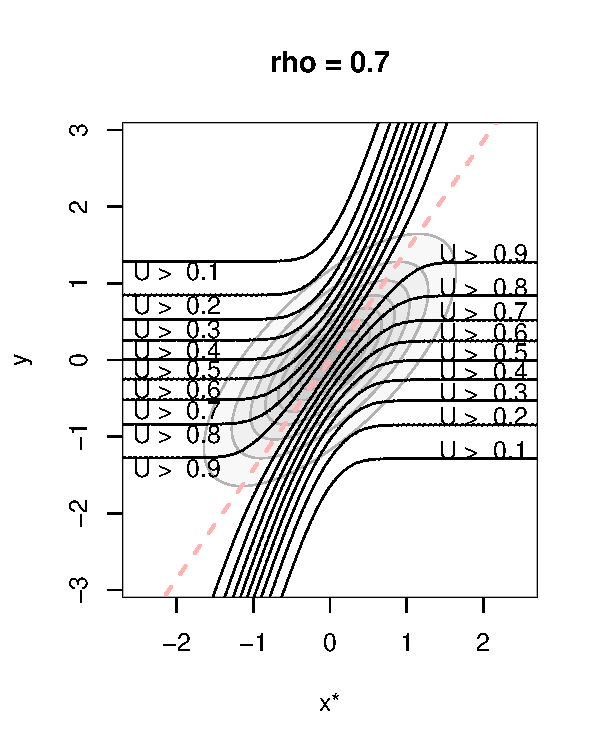
\includegraphics[scale = 0.6, clip = true, trim = 0.1in 0 0 0.8in]{illus_ufunc_0_7.pdf} &
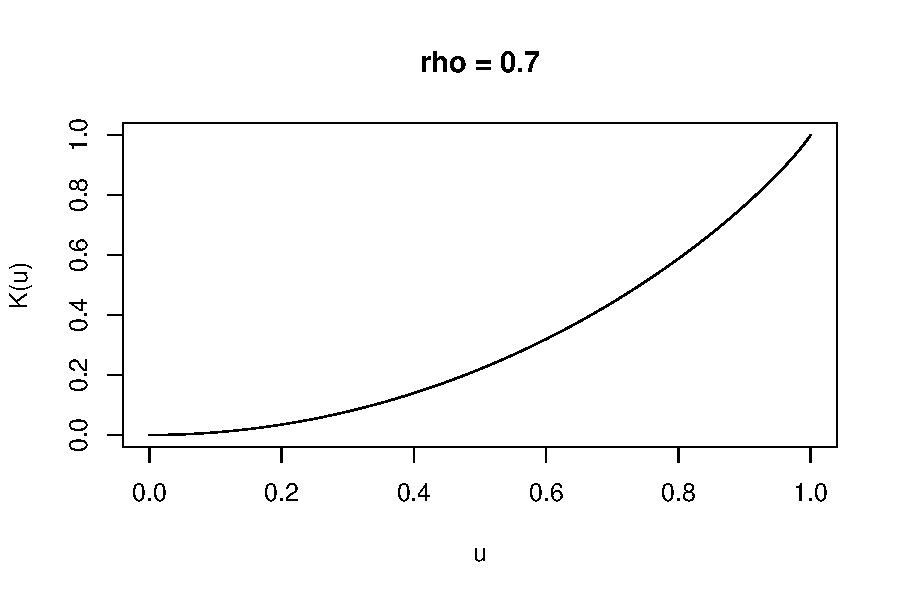
\includegraphics[scale = 0.65, clip = true, trim = 0.22in -0.3in 0 0.5in]{illus_kfunc_0_7.pdf}
\end{tabular}

\caption{\textbf{Favorability for toy example:}
\emph{Left:} The level curves of the function $U_{x^*}(m_y)$ in the bivariate normal model with $\rho = 0.7$.
\emph{Right:} The function ${D}(u)$ gives the cumulative distribution function of the random variable $U_{X^*}(M_Y)$.}\label{fig:toy3}
\end{figure}

It is illuminating to consider how the average accuracy curves and the
${D}(u)$ functions vary as we change the parameter $\rho$.  Higher
correlations $\rho$ lead to higher accuracy, as seen in figure
\ref{fig:toy4}(a), where the accuracy curves are shifted upward as
$\rho$ increases from 0.3 to 0.9.  The favorability $U_{x^*}(m_y)$
tends to be higher on average as well, which leads to lower values of
the cumulative distribution function--as we see in figure
\ref{fig:toy4}(b), where the function ${D}(u)$ becomes smaller as
$\rho$ increases.



\begin{figure}[h]
\centering
\begin{tabular}{cc}
\begin{myfont}\hspace{0.2in}$D(u)$\end{myfont} &
\begin{myfont}\hspace{0.4in}Average Accuracy\end{myfont} \\
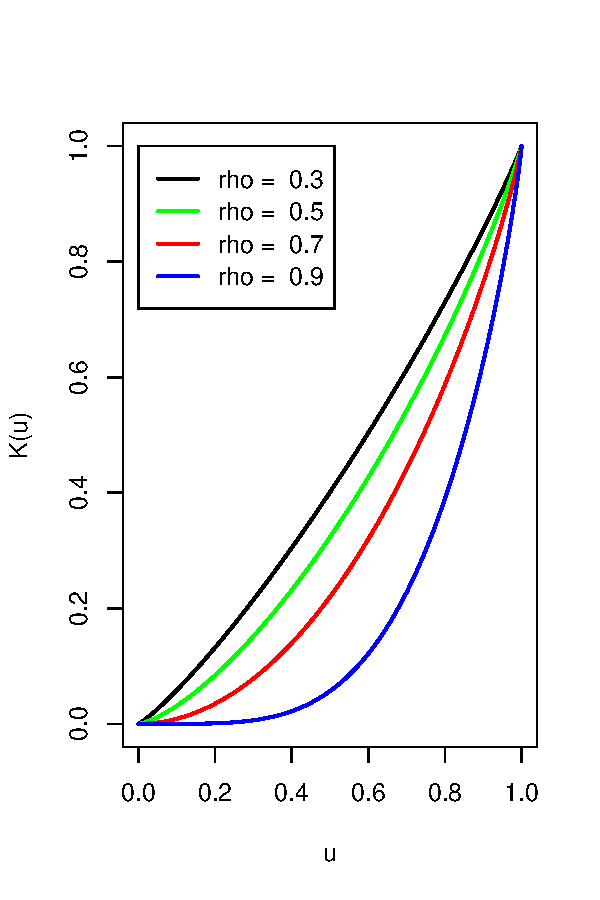
\includegraphics[scale = 0.6, clip = true, trim = 0.22in 0 0.2in 0.6in]{illus_rhos_Kfunc.pdf} &
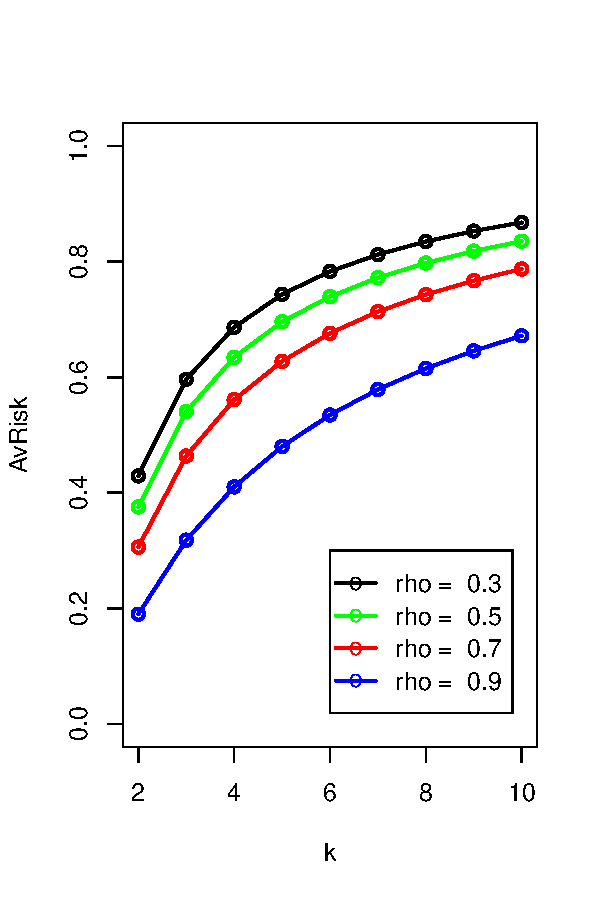
\includegraphics[scale = 0.6, clip = true, trim = 0.0in 0 0.2in 0.6in]{illus_rhos_avrisk.pdf}
\end{tabular}

\caption{\textbf{Average accuracy with different $\rho$'s:}
\emph{Left:} The average accuracy $\text{AGA}_k$. \emph{Right:} ${D}(u)$ function for the bivariate normal model with $\rho \in \{0.3, 0.5, 0.7, 0.9\}$.
}\label{fig:toy4}
\end{figure}

\section{Estimation}\label{sec:extrapolation_estimation}

Next, we discuss how to use data from smaller classification tasks to
extrapolate average accuracy.  Assume that we have data from a
$k_1$-class random classification task, and would like to estimate the
average accuracy $\text{AGA}_{k_2}$ for $k_2>k_1$ classes.  Our
estimation method will use the $k$-class average test accuracies,
$\text{ATA}_2,...,\text{ATA}_{k_1}$ (see Eq \ref{eq:avtestrisk}), for
its inputs.

The key to understanding the behavior of the average accuracy
$\text{AGA}_k$ is the function ${D}$.  We adopt a linear model
\begin{equation}\label{eq:linearKu}
{D}(u) = \sum_{\ell = 1}^m \beta_\ell h_\ell(u),
\end{equation}
where $h_\ell(u)$ are known basis functions, and $\beta_\ell$ are the linear coefficients to be estimated. 

Conveniently, the $\text{AGA}_k$ can also be expressed in terms of the $\beta_\ell$ coefficients.
If we plug in the assumed linear model \eqref{eq:linearKu} into the
identity \eqref{eq:avrisk_identity}, then we get
\begin{align}
1 - \text{AGA}_k &= (k-1)\int {D}(u) u^{k-2} du
\\&= (k-1)\int_0^1 \sum_{\ell = 1}^m \beta_\ell h_\ell(u) u^{k-2} du
\\&= \sum_{\ell = 1}^m \beta_\ell H_{\ell,k} \label{eq:avrisk_linear}
\end{align}
where
\begin{equation}
H_{\ell,k} = (k-1) \int_0^1 h_\ell(u) u^{k-2} du.
\end{equation}
The constants $H_{\ell, k}$ are moments of the basis function
$h_\ell$: hence we call this method the \emph{moment method.}  Note
that $H_{\ell, k}$ can be precomputed numerically for any $k \geq 2$.

Now, since the test accuracies $\text{ATA}_k$ are unbiased estimates
of $\text{AGA}_{k}$, this implies that the regression estimate
\[
\hat{\beta} = \argmin_\beta \sum_{k=2}^{k_1} \left( (1 - \text{ATA}_k) - \sum_{\ell=1}^m \beta_\ell H_{\ell, k}\right)^2
\]
is unbiased for $\beta$. The estimate of $\text{AGA}_{k_2}$ is similarly obtained
from \eqref{eq:avrisk_linear}, via
\begin{equation}\label{eq:avrisk_hat}
\widehat{\text{AGA}_{k_2}} = 1 - \sum_{\ell=1}^m \hat{\beta}_\ell H_{\ell, k_2}.
\end{equation}





\section{Face recognition example}\label{sec:extrapolation_example}

We demonstrate the extrapolation of average accuracy by predicting the
accuracy of a face recognition on a large set of labels from the
system's accuracy on a smaller subset.

\subsection{Data}
From the ``Labeled Faces in the Wild'' dataset (\cite{LFWTech}), we
selected the 1672 individuals with at least 2 face photos.  We form a
dataset consisting of photo-label pairs $(x_j^{(i)}, y^{(i)})$
for $i = 1,\hdots, 1672$ and $j = 1,2$ by randomly selecting 2 face
photos for each individual. 

\begin{figure}
\centering
\begin{tabular}{|c|ccc|c|}
\hline
Label & & Training & & Test\\ \hline
$y^{(1)}$=Amelia & 
  $x_1^{(1)} = $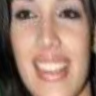
\includegraphics[scale = 0.2]{face_photos/Amelia_Vega_0001.png} &  
  $x_2^{(1)} = $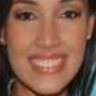
\includegraphics[scale = 0.2]{face_photos/Amelia_Vega_0002.png} &  
  $x_3^{(1)} = $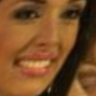
\includegraphics[scale = 0.2]{face_photos/Amelia_Vega_0003.png} &  
  $x_*^{(1)} = $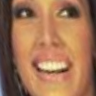
\includegraphics[scale = 0.2]{face_photos/Amelia_Vega_0004.png} \\ \hline
$y^{(2)}$=Jean-Pierre & 
  $x_1^{(2)} = $
\includegraphics[scale = 0.2]{face_photos/Jean-Pierre_Raffarin_0001.png} &  
  $x_2^{(2)} = $
\includegraphics[scale = 0.2]{face_photos/Jean-Pierre_Raffarin_0002.png} &  
  $x_3^{(2)} = $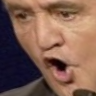
\includegraphics[scale = 0.2]{face_photos/Jean-Pierre_Raffarin_0003.png} &  
  $x_*^{(2)} = $
\includegraphics[scale = 0.2]{face_photos/Jean-Pierre_Raffarin_0004.png} \\ \hline
$y^{(3)}$=Liza & 
  $x_1^{(3)} = $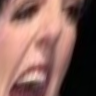
\includegraphics[scale = 0.2]{face_photos/Liza_Minnelli_0001.png} &  
  $x_2^{(3)} = $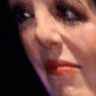
\includegraphics[scale = 0.2]{face_photos/Liza_Minnelli_0002.png} &  
  $x_3^{(3)} = $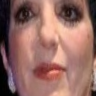
\includegraphics[scale = 0.2]{face_photos/Liza_Minnelli_0003.png} &  
  $x_4^{(3)} = $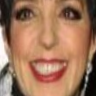
\includegraphics[scale = 0.2]{face_photos/Liza_Minnelli_0004.png} \\ \hline
$y^{(4)}$=Patricia & 
  $x_1^{(4)} = $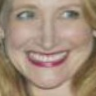
\includegraphics[scale = 0.2]{face_photos/Patricia_Clarkson_0001.png} &  
  $x_2^{(4)} = $
\includegraphics[scale = 0.2]{face_photos/Patricia_Clarkson_0002.png} &  
  $x_3^{(4)} = $
\includegraphics[scale = 0.2]{face_photos/Patricia_Clarkson_0003.png} &  
  $x_4^{(4)} = $
\includegraphics[scale = 0.2]{face_photos/Patricia_Clarkson_0004.png} \\ \hline
\end{tabular}
\caption{\textbf{Face recognition setup:} Examples of labels and features from the \emph{Labeled Faces in the Wild} dataset.}
\label{fig:face_rec}
\end{figure}

\subsection{Classifier}
We implement a two-step face recognition system based on a precomputed neural-network based embedding followed by a one nearest neighbor classifier.

We used the OpenFace (\cite{amos2016openface}) embedding for feature
extraction.  For each photo $x$, a 128-dimensional feature vector
$g(x)$ is obtained as follows.  The computer vision library DLLib is
used to detect landmarks in $x$, and to apply a nonlinear
transformation to align $x$ to a template.  The aligned photograph is
then downsampled to a $96 \times 96$ image. The downsampled image is
fed into a pre-trained deep convolutional neural network to obtain the
128-dimensional feature vector $g(x)$. More details are found in
(\cite{amos2016openface}).

The recognition system then works as follows.  Suppose we want to
perform facial recognition on a subset of the individuals, $I \subset
\{1,\hdots, 1672\}$.  Then, for all $i \in I$, we load one example-label pair, into the system, $(x_1^{(i)}, y^{(i)})$.  In
order to identify a new photo $\vec{z}^*$, we obtain the feature
vector $g(x^*)$, and guess the label $\hat{y}$
with the minimal Euclidean distance between $g(y^{(i)})$ and $g(x^*)$,
which implies a score function
\[
M_{y^{(i)}}(x^*) = -||g(x_1^{(i)}) - g(x^*)||^2.
\]


The test accuracy is assessed on the unused repeat for all individuals
in $I$.  Note that the assumptions of our estimation method are met in
this example because one-nearest neighbor is a marginal classifier.
We note that $m$-nearest neighbor for $m > 1$ is not marginal.

\subsection{Experimental Details}\label{sec:exp_details}
We treat the full data-set of $1672$ as our population of labels. In
each experiment, we choose a random subset of size $k_1<1672$, for
which we observe both training and test data. From this data, we will
estimate $\text{AGA}_{k_2}$ for $k_2$ between $k_2 =
k_1+1,...,1672$. We use $k_1 = 100,200,400,800$, with $B = 300$
repeats for each subset size.

For the selected subset of size $k_1$, we can estimate the test
accuracy at every $k \leq k_1$, getting the vector
$(\text{ATA}_2,...,\text{ATA}_{k_1})$.  Specifically, we use a linear
spline basis,
\[
h_\ell(u) = \left[u - \frac{\ell}{m + 1}\right]_+
\]
for $\ell = 1,\hdots, m$.  Here we take $m = 10000$. 
We fit the $\beta$ coefficient vector using non-negative least squares: 
\[
\hat{\beta} = \argmin_{\beta: \beta_\ell \geq 0} \sum_{k=2}^{k_1} \left( (1 - \text{ATA}_k) - \sum_{\ell=1}^m \beta_\ell H_{\ell, k}\right)^2
\]
The non-negativity constraint on the coefficients $\beta$, combined
with the linear spline basis, ensures that ${D}(u)$ is a monotonic
and convex function on $[0,1]$.

Based on the $\beta$ coefficients, we can compute the prediction for
the full dataset $\hat{AGA}_{1672}$.  We compare the prediction to the
observed accuracy on full dataset $\text{TA}_{1672}$, which
approximates the ground truth.


\begin{figure}
\centering
\begin{tabular}{c}
\begin{myfont}Predicting $\text{AGA}$ ($k_1= 400$) \end{myfont}\\
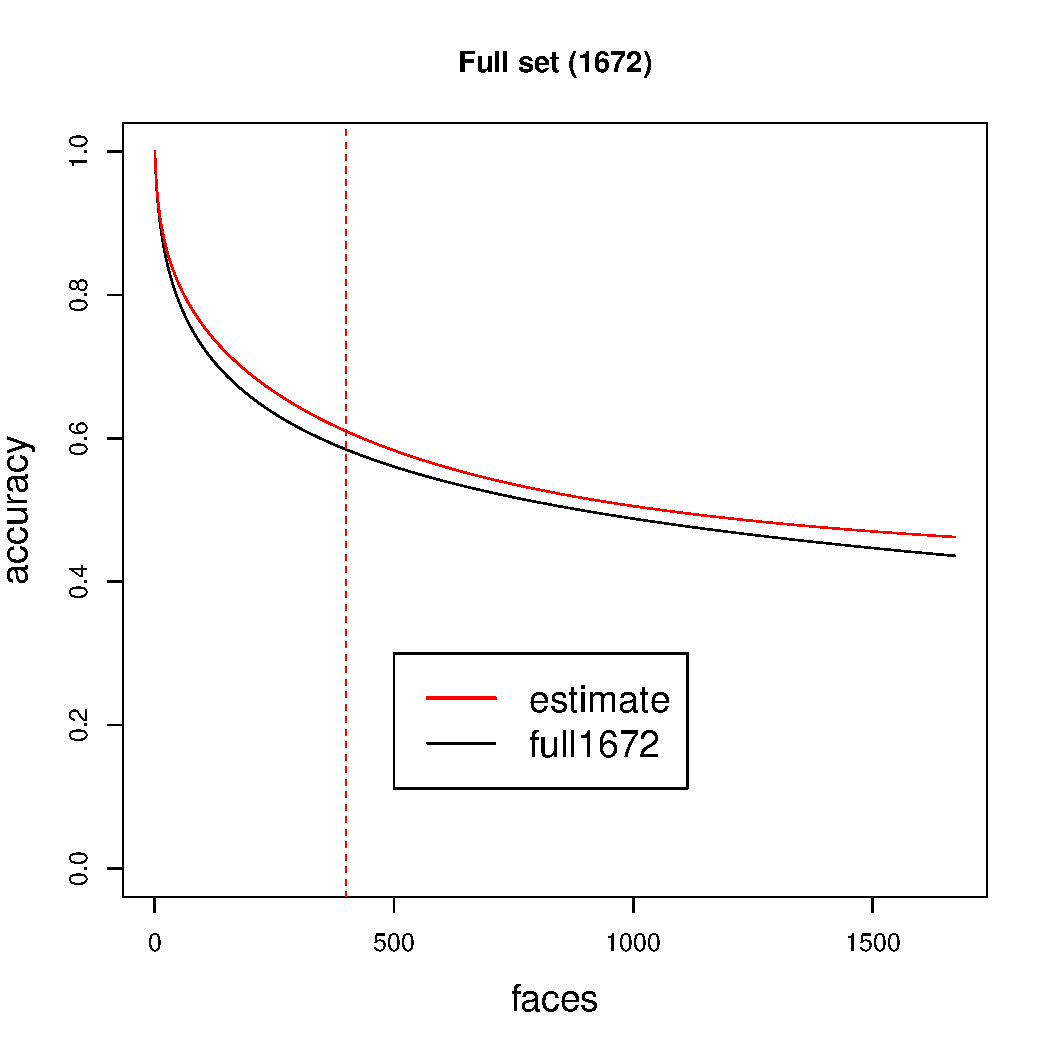
\includegraphics[scale = 0.5, clip = true, trim = 0 0 0 0.6in]{acc_plot2.pdf}
\end{tabular}
\caption{\textbf{Estimated accuracy for face recognition:}
Estimated average accuracy for $k > 400$ (red) compared to the ground truth (blue). Estimation is based on observed accuracies using one subset of $k_1=400$ classes (black), whereas ground truth uses all 1672 classes. The results are for 1-NN classifier.}
\label{fig:lfw_extrapolation1}
\end{figure}

\subsection{Results}

The extrapolation results can be seen in Figures
\ref{fig:lfw_extrapolation1} and \ref{fig:lfw_extrapolation2}. In the
first, we show a extrapolation estimate for $k_1 = 400$. In the
second, we see multiple instances for different values of $k_1$. As
can be seen, both the accuracy as well as the variances decrease
rapidly as $k_1$ increases. In general, for $k_1>400$ the paths of the
different extrapolation curves are not very different. The
root-mean-square errors between at $k_2=1672$ can be seen in Table
\ref{tab:lfw_accuracy}.

\begin{figure}
\centering
\begin{tabular}{cc}
\begin{myfont}$k_1 = 100$\end{myfont} & 
\begin{myfont}$k_1 = 200$\end{myfont}\\
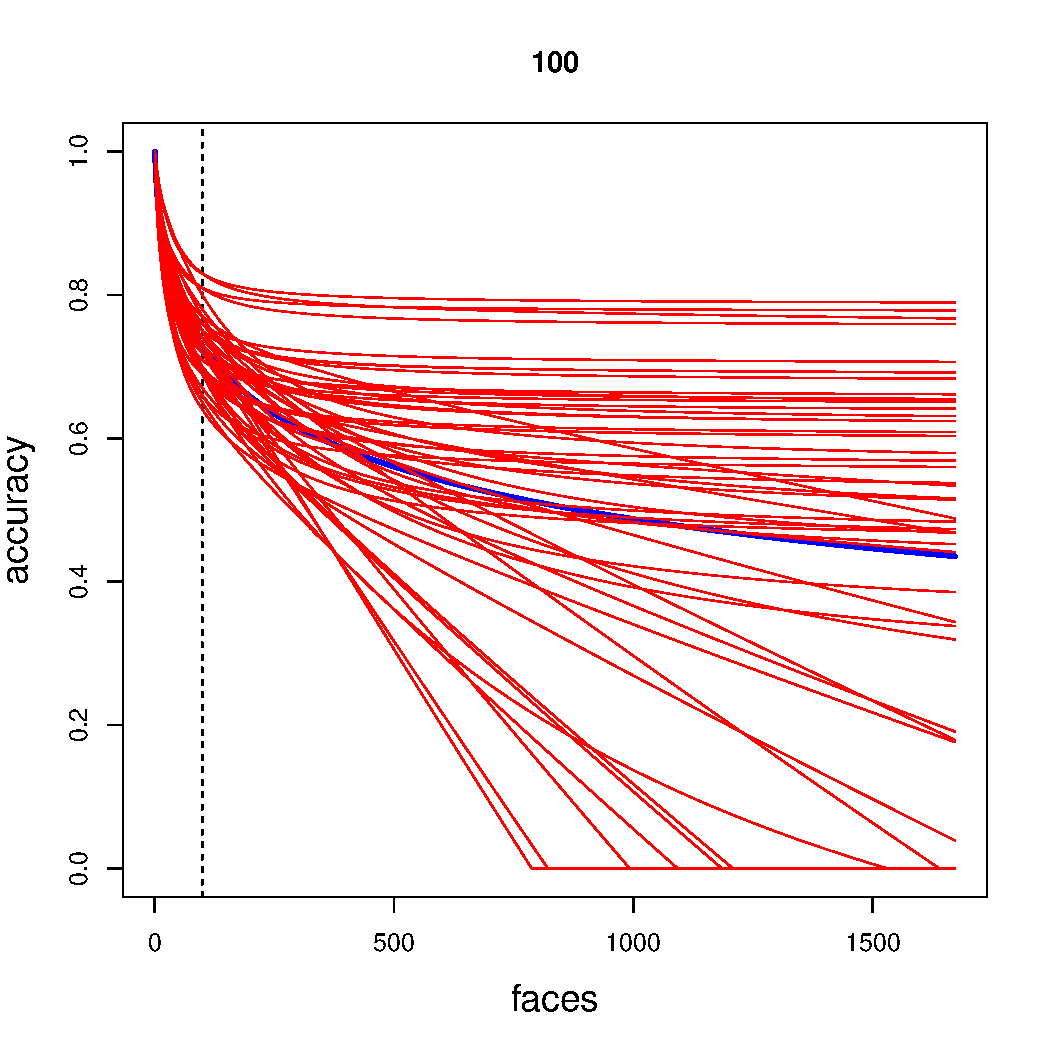
\includegraphics[scale = 0.4, clip = true, trim = 0 0 0 0.6in]{sub_100.pdf} &
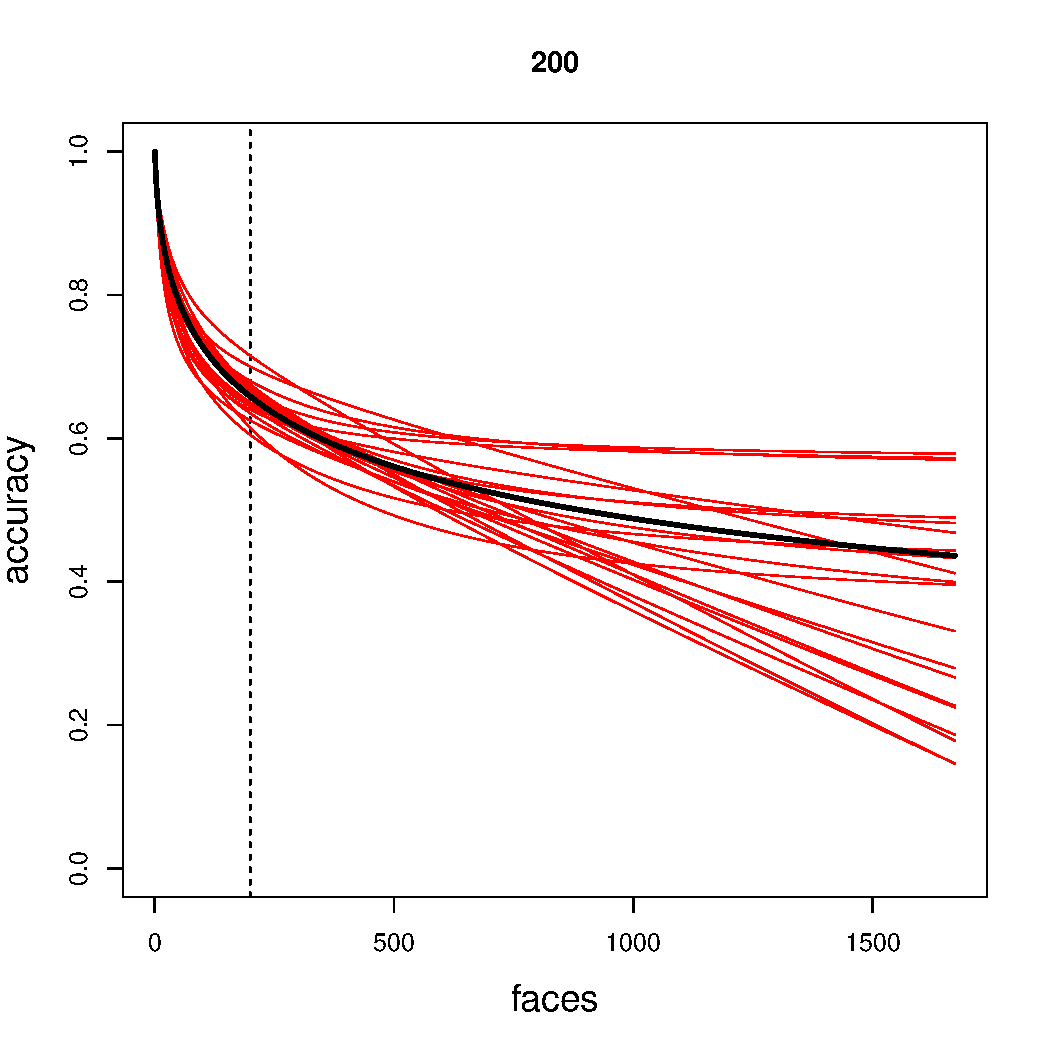
\includegraphics[scale = 0.4, clip = true, trim = 0 0 0 0.6in]{sub_200.pdf} \\
\begin{myfont}$k_1 = 400$\end{myfont} & 
\begin{myfont}$k_1 = 800$\end{myfont}\\
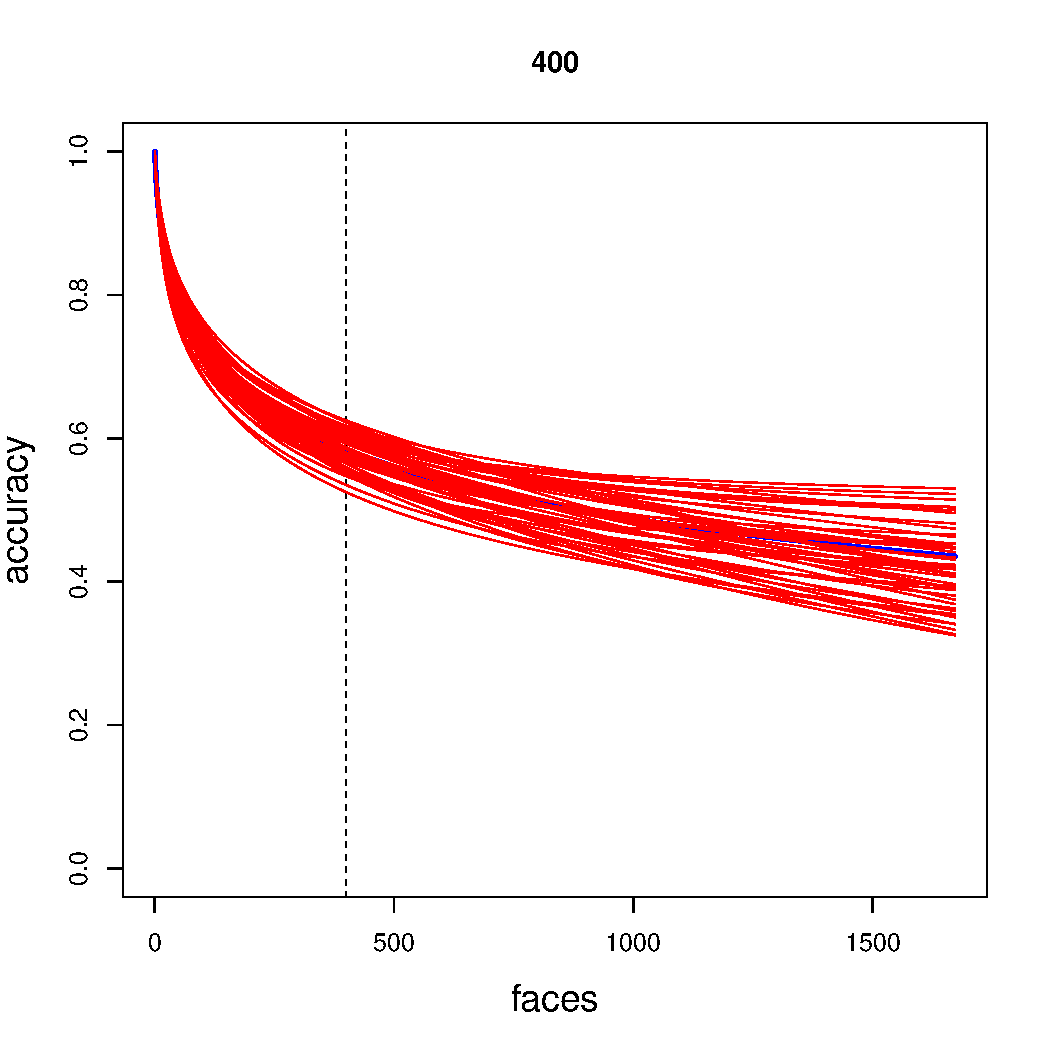
\includegraphics[scale = 0.4, clip = true, trim = 0 0 0 0.6in]{sub_400.pdf} &
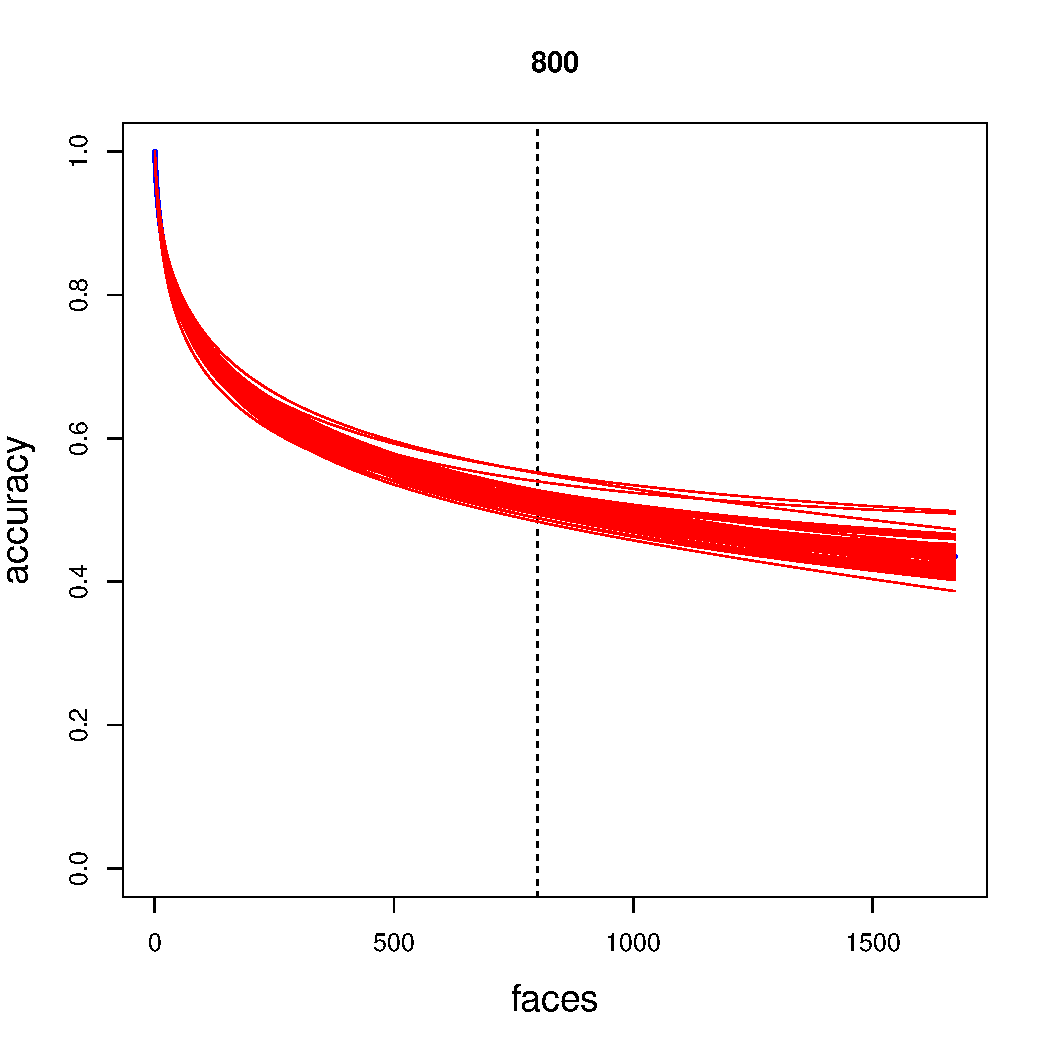
\includegraphics[scale = 0.4, clip = true, trim = 0 0 0 0.6in]{sub_800.pdf} 
\end{tabular}
\caption{\textbf{Comparing different $k_1$s:}
The plots show predicted accuracies using a different source dataset size $k_1$ (vertical line). Each red curve represents the estimated accuracies using a single subsample. The black curve shows the true average accuracy. }
\label{fig:lfw_extrapolation2}
\end{figure}

\begin{table}
\centering
\begin{tabular}{c||c|c|c|c}
\hline
$k_1$ & 100 & 200 & 300 & 400 \\\hline
Bias & -0.090 & -0.062 & -0.016 & -0.001\\\hline
sd & 0.277 & 0.178 & 0.066 & 0.020 \\ \hline
RMSE & 0.291 & 0.189 & 0.068 & 0.020 \\\hline
\end{tabular}
\caption{Bias, standard deviation, and RMSE on predicting $\text{TA}_{1672}$ from $\widehat{\text{AGA}_{k_1}}$}\label{tab:lfw_accuracy}
\end{table}

\section{Simulation study}\label{sec:simulation_study}

We ran simulations to check how the proposed extrapolation method performs in different settings.  The results are displayed in Figure \ref{fig:sim_study}. We varied the number of classes $k_1$ in the source dataset, the difficulty of classification, and the basis functions. We generated data according to a mixture of isotropic multivariate Gaussian distributions: labels $Y$ where sampled from $Y \sim N(0, I_{10})$, and the examples for each label sampled from $X|Y \sim N(Y, \sigma^2 I_{10})$. $\sigma$ is a noise-level parameter that determines the difficulty of classification. Similarly to the real-data example, we consider a 1-nearest neighbor classifier, which is given a single training instance per class. In all simulations, we predict the average accuracy for $k = 2000$ classes. We vary  $k_1$, the number of classes in the source task; and $\sigma$, which controls the noise level, and hence the true average accuracy.

For the estimation, we compare several spline bases, all of the form $h_\ell(u) = [u - t_\ell]_+$ for some set of knots $\{t_\ell\}_{\ell = 1}^m$. Spline bases vary by the number and the spacing of knots: 
\begin{itemize}
\item \emph{linear spacing} chooses knots according to
\[
t_\ell = \frac{\ell}{m+1}.
\]
\item \emph{quadratic spacing}  has an increased density of knots near 1
\[
t_\ell = \left(1 - \frac{m + 1 -\ell}{m+1}\right)^2.
\]
\end{itemize}

The rationale for increasing the density of knots near 1 is that
when attempting to extrapolate to a large number of
classes, the behavior of ${D}(u)$ for $u$ close to 1 is far more
important than the shape of ${D}(u)$ in the rest of the interval.
This is because the weighting density $\text{Beta}(k-1, 1)$ used to
compute the higher moments is concentrated near 1 for large $k$.


We compare linear and quadratic spacings for spline bases of size $m = \{100,1000,10000\}$.
For all spline bases, we fit the coefficients using a non-negativity constraint on $\beta$, 
which enforces convexity of the estimated $\hat{D}(u).$

\subsection*{Results}
In Figure \ref{fig:sim_study} (top right) we see how the accuracy of prediction
improves as we increase the number of classes in the training set, $k_1=\{50,\hdots,2000\}$, while fixing $\sigma = 0.55$.
We see that the performance curves of most spline bases is similar. An outlier is the spline basis with linear spacing and $m=100$ ({\tt lin2}). This case enjoys better RMSE for $k_1 < 150$; however, for $k_1 > 400$ the main group has far better extrapolation performance.
A possible explanation for the relatively poor performance of the {\tt lin2} is that this basis cannot approximate the true $D(u)$ function (bottom left of figure) to a sufficiently high resolution.
When the source dataset too small to accurately fit $D(u)$, such as when $k_1 < 150$, this may not be a disadvantage. But as more data becomes available and the variance of estimation
decreases, models with lower bias obtain better results.
Note that quadratic spacing with the same number of knots ($m=100$) matches the performance of much larger spline bases.  This suggests that a small spline basis with $m << k_1$ can perform almost as well as an optimally sized spline basis, as long as appropriate spacing is used.
 
In the bottom right of Figure \ref{fig:sim_study}, we fix $k_1=500$ and vary $\sigma=\{0.3,\hdots,0.7\}$. This allows us to evaluate the reliability of the extrapolation across a wide range of possible signal-to-noise ratios.
The true average accuracy $\text{AGA}_{2000}$ varies from 0.838 for $\sigma = 0.3$ to 0.102 for $\sigma = 0.7$.
In this case, the spline bases can be divided into three groups.
Once again, {\tt lin2} forms a group by itself--the worst performing group, but {\tt lin3} with $m = 1000$ linearly spaced knots is also alone in the best group, and the other spline bases form the third group performing similarly to {\tt lin3}.
We do not currently have an explanation of why {\tt lin3} has the best performance across all noise levels.




\begin{figure}
\centering
\begin{tabular}{cc}
\begin{myfont}Predicting $\text{AGA}_{2000}$ from $k_1 = 500$\end{myfont} &
\begin{myfont}Error versus $k_1$ ($\sigma = 0.55$)\end{myfont}\\
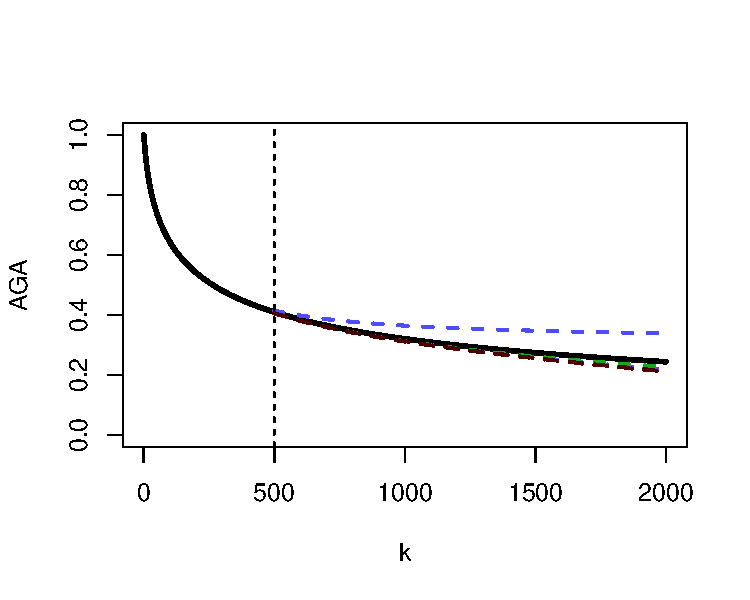
\includegraphics[scale = 0.55, clip = true, trim = 0 0 0 0.6in]{mcgs2_oneplot.pdf} &
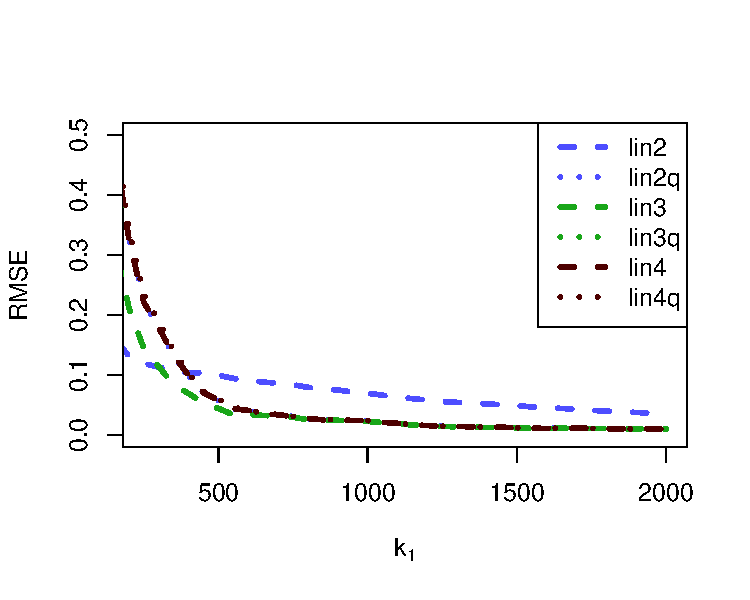
\includegraphics[scale = 0.55, clip = true, trim = 0 0 0 0.6in]{fig_mcgs2f.pdf}\\
\begin{myfont}Simulated $D(u)$ functions\end{myfont} &
\begin{myfont}Error versus $\sigma$ ($k_1 = 500$)\end{myfont}\\
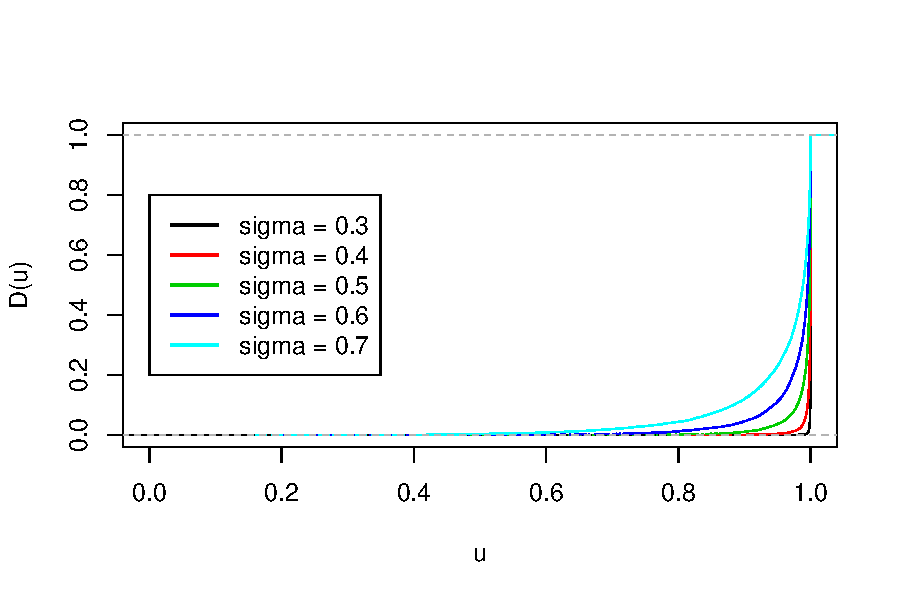
\includegraphics[scale = 0.55, clip = true, trim = 0 0 0 0.6in]{fig_mgs2.pdf} &
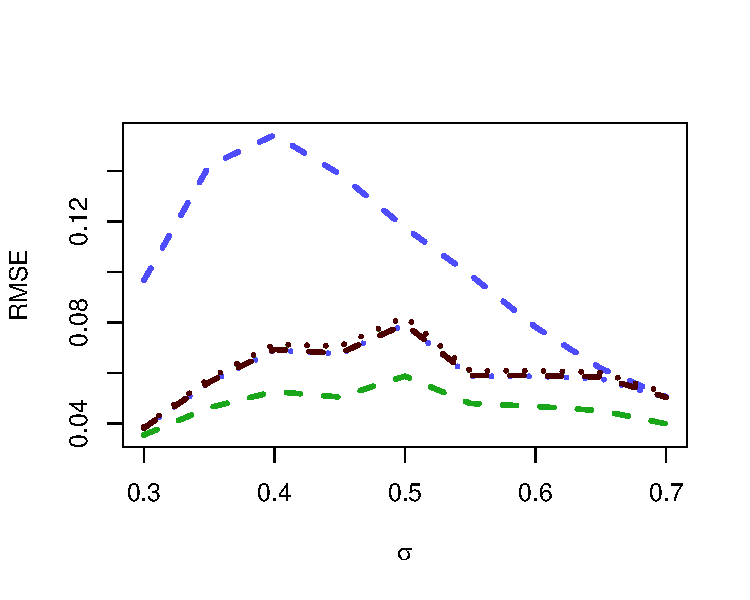
\includegraphics[scale = 0.55, clip = true, trim = 0 0 0 0.6in]{fig_mcgs2fovs_02.pdf}\\ 
\end{tabular}
\caption{\textbf{Simulation results:}
 Simulation study consisting of multivariate Gaussian $Y$ with nearest neighbor classifier.  Comparison of various linear spline bases for extrapolation,
  in multivariate Gaussian simulation with $Y \sim N(0, I_{10})$, $X|Y
  \sim N(Y, \sigma^2 I_{10})$, and $r=1$ training set.  The spline
  bases are lin2 (100 knots), lin3 (1000 knots) and lin4 (10000) knots
  with uniform knot spacings from [0,1], and lin2q, lin3q, and lin4q
  are corresponding bases with quadratic spacing of knots (more
  densely packed near 1).  \emph{Top left:} Extrapolating from $k_1 = 500$ up to $k
  = 2000$ compared to true accuracy, with $\sigma = 0.55$. \emph{Top right:} The
  RMSE of $\widehat{\text{AGA}_{2000}}$ for varying $k_1$ and $\sigma
  = 0.55$. \emph{Bottom right:} The actual distribution functions
  $D(u)$ for varying $\sigma$.} \emph{Bottom left:} The RMSE of $\widehat{\text{AGA}_{2000}}$ for $k_1 = 500$ and varying $\sigma$. 
\label{fig:sim_study}
\end{figure}


\section{Discussion}
\label{sec:discussion}
In this work, we suggest treating the class set in a classification
task as random, in order to extrapolate classification performance on
a small task to the expected performance on a larger unobserved task.
We show that average generalized accuracy decreases with increased
class-set size like the $(k-1)$th moment of a distribution function.
Furthermore, we introduce an algorithm for estimating this underlying
distribution, that allows efficient computation of higher order
moments.  There are many choices and simplifying assumptions used in
the description of the method.  In this discussion, we discuss these
decisions and map some alternative models or strategies for future
work.



\subsubsection*{Fitting  ${D}(u)$}
Estimation accuracy of ${D}(u)$ will depend on how well it is
approximated by basis functions $h_\ell(u)$, and penalty and
constraints used for fitting the regression.  Based on our experience
with simulated and real data examples, we can offer a couple of
practical suggestions for the fitting procedure.

\begin{itemize}
\item Although ${D}(u)$ is unknown, it has to be monotone and bounded by one,
because it is a cumulative distribution function.  Furthermore, in
many real and simulated examples, including the examples of sections \ref{sec:simulation_study} and \ref{sec:extrapolation_example},
${D}(u)$ also has the property
of convexity.  We have found that including the monotonicity and
convexity constraint in the estimation procedure improves estimation
performance.  A convenient way to impose both is to choose $\{h_\ell\}$ to be a family of
linear splines, $h_\ell(u) = [u - u_\ell]_+$, and then to require that
the spline coefficients $\beta_\ell$ are non-negative (see Section \ref{sec:exp_details}). 
We expect that higher-order spline
bases should also do well, although it may be harder to impose the 
convexity and monotonicity constraints.
\item The number and location of knots for the spline basis is also
important.  
%When attempting to extrapolate to a large number of
%classes, the behavior of ${D}(u)$ for $u$ close to 1 is far more
%important than the shape of ${D}(u)$ in the rest of the interval.
%This is because the weighting density $\text{Beta}(k-1, 1)$ used to
%compute the higher moments is concentrated near 1 for large $k$.  A
%good heuristic is to consider that the mean of the weighting density
%is $\frac{k-1}{k}$, which suggests that the scale of discretization
%near 1 should be smaller than $1/k_2$ when the goal is to estimate the
%average accuracy for $k_2$ classes.  Meanwhile, the standard deviation
%of the weighing density is approximately $1/k$, meaning that the
%behavior of ${D}(u)$ for $u$ smaller than $1 - \frac{5}{k_2}$
%(that is, $u$ which are more than 4 standard deviations away from the
%mean of the weighting density) has negligible effect on the
%extrapolation.  Therefore, a coarser discretization can be used for
%knots while are smaller than $1 - \frac{5}{k_2}$.  Still, the overall
%discretization should not be coarser than order $1/k_1$, so that the
%model has sufficient degrees of freedom to explain the subsampled
%accuracy curve. 
We found that controlling the number of basis functions is crucial for preventing overfitting in the unconstrained linear model. When
at least one of either the monotonicity or convexity constraint is
adopted, however, the fit is less sensitive to the number of basis
functions, as long as the knots form a sufficiently fine
discretization of the unit interval.  Even then, careful choice of knots can reduce the computational load.
\item An alternative to a linear basis representation is to
consider parametric families for the function ${D}(u)$.  When the
family is a good fit to the the data, this can considerably improve
extrapolation power, especially when the size of the dataset is
limited.  We discuss parametric models for ${D}(u)$ in
forthcoming work.
\end{itemize}

\subsubsection*{Comparison to Kay et al.}
The extrapolation method of \cite{Kay2008a} can be described in our
framework as follows.  Let $F_x$ be the cumulative distribution
function of $M_{Y'}(x)$ for a random label $Y' \sim \pi$.  For each
test instance $x^{(i)}_j$, let
$\hat{F}_{x^{(i)}_j}(m_{y^{(i)}}(x^{(i)}_j))$ be an estimate of
$F_{x^{(i)}_j}(m_{y^{(i)}}(x^{(i)}_j))$.  The particular estimation
method recommended by \citep{Kay2008a} is to estimate the density
$f_{x^{(i)}_j}$ by using kernel-density estimation with a Gaussian
kernel and a bandwidth chosen via pseudolikelihood cross-validation
\citep{cao1994comparative}; however, our criticism is not specific to
the use of a particular estimator for $\hat{F}_x$.  Extrapolate using
the formula
\[
\widehat{\text{AGA}_k} = \frac{1}{k_1 r} \sum_{i=1}^k \sum_{j=1}^r \hat{F}_{x^{(i)}_j}(m_{y^{(i)}}(x^{(i)}_j))^{k-1}
\]
While no justification is given for the method in (\cite{Kay2008a}),  one possible justificiation is the fact that
\[\text{AGA}_k = \E[F_X(M_{Y}(X))^{k-1}].\]
Therefore, the method can give good extrapolations when the estimated
probabilities $\hat{F}_{x^{(i)}_j}(m_{y^{(i)}}(x^{(i)}_j))$ are close
to the true probabilities $F_{x^{(i)}_j}(m_{y^{(i)}}(x^{(i)}_j))$.
However, the method ignores the bias introduced by exponentiation.
That is, even if $\hat{p}$ is an unbiased estimator of $p$, $\hat{p}^k$ may \emph{not} be a very good estimate of $p^k$, since
\[
p^k = \E[\hat{p}]^k \neq \E[\hat{p}^k].
\]
unless $\hat{p}$ is a degenerate random variable
(constant). Otherwise, for large $k$, $\hat{p}^k$ may be an extremely
biased estimate of $p$.  Our proposed method avoids this source of
bias by estimating the $(k-1)$st moment of $D(u)$ directly.

\subsubsection*{Marginal classifiers}
One limitation of our analysis of average accuracy is that it applies
only to marginal classifiers.  Theoretically, it may be possible to
extend the analysis to certain non-marginal classifiers, for instance,
by showing that in the large-$k$ limit such classifiers become
``asymptotically'' marginal, in some sense. Furthermore,  
there is no obstacle in testing the extrapolation method to
see how well it would recover accuracy curves for non-marginal classifiers. 

\subsubsection*{Sampling}
Our analysis is currently restricted to
randomized classification problems with i.i.d. sampling of classes.
Extension to other sampling mechanisms, such as cluster sampling, may
be possible if one can work out how the dependence between classes
translates into dependence between the favorabilities
$U_{X^*}(m_{Y^{(k)}})$. 

More broadly, the assumption that the labels in $\mathcal{S}_k$ are a
random sample from a distribution $\pi$ may be inappropriate.  Many
natural classification problems arise from hierarchically partitioning
a space of instances into a set of labels.  Therefore, rather than
modeling $\mathcal{S}_k$ as a random sample, it may be more suitable
to model it as a random hierarchical partition of $\mathcal{Y}$ (for
instance, arising from an optional P{\'o}lya tree process,
\cite{wong2010optional}).
Finally, note that we assume no knowledge about the new class-set
except for its size. Better accuracy might be achieved if some partial information 
is known.

\subsubsection*{Arbitrary cost functions}

In the current paper, we only discussed extrapolating the
classification accuracy--or equivalently, the risk for the zero-one
cost function.  However, it is possible to extend our analysis to risk
functions with arbitrary cost functions, which is the subject of
forthcoming work.

\subsubsection*{Predicting the generalization accuracy}
In this work, our focus was on estimating the average generalization accuracy.  However, rather being interested in the average accuracy for a new label set, one might be interested in predicting the generalization accuracy on a particular problem.  When the source task and target tasks are independent, then the average generalization accuracy is also Bayes estimate which minimizes mean-squared prediction error.  However, it may be known that there is overlap between the labels or data used in the source task or target task.  Conditioning on this information may yield a more accurate prediction.  However, we leave this problem to future work.

\subsubsection*{Confidence and prediction intervals}
In many of the applications discussed in the introduction, it would be useful to construct either confidence intervals for the average generalization accuracy $\text{AGA}_k$, or prediction intervals for the generalization accuracy, $\text{GA}_k$.
The key to constructing such intervals is to understand the variability properties of the inputs to our estimation procedure, the average test accuracies $\text{ATA}_k$.  We discuss the issue of constructing confidence and prediction intervals in forthcoming work.

\subsubsection*{Other transfer learning setups}
In our analysis, we also limited the training set sizes to be the same in both the source and target tasks.  It would be very nice to be able to relax this assumption, since in most practical applications, the training set sizes are varied within label sets as well as between tasks.  The idea of extrapolating from learning curves \citep{cortes1994learning} may be one way to adjust for varying training set sizes.  


Many other aspects of transfer learning could also be considered in
conjunction with the issue of transferring from one label set to
another, such as transfer to a different domain, or transfer to a
target task without training data \citep{pan2010survey}. 

% \begin{itemize}
% \item Basis function (and convexity)
% \item Parametric models
% \item Non-marginal classifiers
% \item Sampling mechanisms
% \item Hierarchical setup: K increases, but not sampling rather partitioning
% \item Other cost functions (Current Work)
% \item Differing training set sizes (cortes)
% \item Other aspects of transfer learning
% \end{itemize}
 

\acks{We thank Jonathan Taylor, Trevor Hastie, John Duchi, Steve
  Mussmann, Qingyun Sun, Robert Tibshirani for useful discussion.  CZ
  is supported by an NSF graduate research fellowship, and would also
  like to thank the European Research Council under the ERC grant agreement n° [PSARPS-294519]  for travel support.
}

\bibliography{example}

\end{document}

